\documentclass[hidelinks]{article}
\usepackage[a4paper, total={7in, 10in}]{geometry}
\usepackage[dvipsnames]{xcolor}
\usepackage{amsmath}
\usepackage{tikz}
\usepackage{tkz-euclide}
\usepackage[unicode]{hyperref}
\usepackage[all]{hypcap}
\usepackage{fancyhdr}
\usepackage[UTF8,fontset=fandol]{ctex}
\usepackage{graphicx}
\usepackage{float}

\usetikzlibrary{angles,calc, decorations.pathreplacing}

\newcommand{\dps}{\displaystyle}
\newcommand{\vt}[1]{\mathbf{#1}}
\newcommand{\norm}[1]{\| #1 \|}
\newcommand{\andd}{\mbox{ and }}
\newcommand{\nott}{\mbox{ not }}
\newcommand{\orr}{\mbox{ or }}
\definecolor{carminered}{rgb}{1.0, 0.0, 0.22}
\definecolor{capri}{rgb}{0.0, 0.75, 1.0}
\definecolor{brightlavender}{rgb}{0.75, 0.58, 0.89}

\title{\textbf{Project 1 REPORT: Solar Eclipse Prediction}}
\author{刘任达\\盛文哲\\蒋弘杰}
\date{March 24th, 2025}
\begin{document}
\hypersetup{bookmarksnumbered=true,}
\maketitle
\setcounter{tocdepth}{2}
\begin{Large}
\tableofcontents
\end{Large}%
\pagebreak

\section{背景介绍}
日食与月食作为人类历史上最引人注目的天体现象之一,不仅是天文学研究的重要对象,更承载着文化、历史和科学探索的多重意义。从古代巴比伦的"沙罗周期"到现代天体力学的高精度数值模拟,人类对日月食的预测始终是连接数学、物理学与天文学的前沿课题。本文致力于运用数学建模与数值分析的严谨方法,在经典天体力学框架下探索多体问题的复杂性,并尝试以创新的技术手段提升预测精度。

在理论层面,日月食的发生本质上是地月系轨道运动与太阳几何关系的周期性呈现。(见图\ref{fig:eclipse})自牛顿建立万有引力定律以来,二体问题的解析解为天体轨道计算奠定了基础,但实际天文系统中的引力摄动效应(如木星等大质量天体的影响)使得问题迅速复杂化。传统日月食预测多基于简化模型(如忽略高阶摄动项或采用经验周期修正),这类方法虽能提供定性规律,却难以满足高精度、长周期的预测需求。因此,如何构建兼顾计算效率与精度的多体动力学模型,成为天体力学数值模拟领域的重要挑战。

\begin{figure}[htbp]
    \centering
    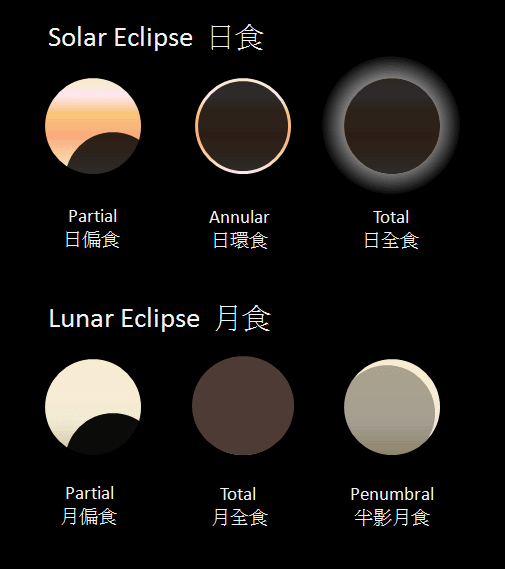
\includegraphics[width=0.5\linewidth]{images/ecltype.png}
    \caption{日月食的种类和图像}
    \label{fig:eclipse}
\end{figure}

本文工作的核心目标是通过建立包含太阳、地球、月球及木星的四体动力学模型,结合四阶龙格-库塔(Runge-Kutta)数值积分方法,实现未来50年内日月食事件类型与发生时刻的高精度预测。选择四阶龙格-库塔方法,源于其对微分方程初值问题的高精度求解特性——该方法通过多步加权平均策略有效抑制局部截断误差,在保证计算稳定性的同时,能够适应地月系轨道长期演化中摄动力引起的非线性效应。在太阳系(见图\ref{})这一复杂引力系统中,太阳作为中心天体占据总质量的99.86\%,而行星际引力作用通过轨道共振与长期摄动深刻影响着各天体的运动轨迹。尽管传统日月食预测模型通常将太阳、地球、月球视为孤立三体系统,但本课题通过第二部分理论分析中的误差量化研究发现:若忽略木星这一太阳系最大行星(质量占行星总质量的60\%)的引力作用,在50年时间尺度上,地月轨道半长轴将产生约$10^{-4}AU$量级的系统性偏移,其累积效应足以导致日月食时刻预测出现分钟级偏差。这种偏差源于木星虽距离地月系约$4.2-6.2$AU,但其$1.9×10^{27}$kg的巨大质量通过引力势的二阶项对地月轨道产生周期性摄动,其影响强度经计算可达$10^{-5}$量级(见\ref{object_error}对象误差)。因此,构建包含木星的四体模型是还原太阳系真实动力学图景的必要举措.

\begin{figure}[htbp]
    \centering
    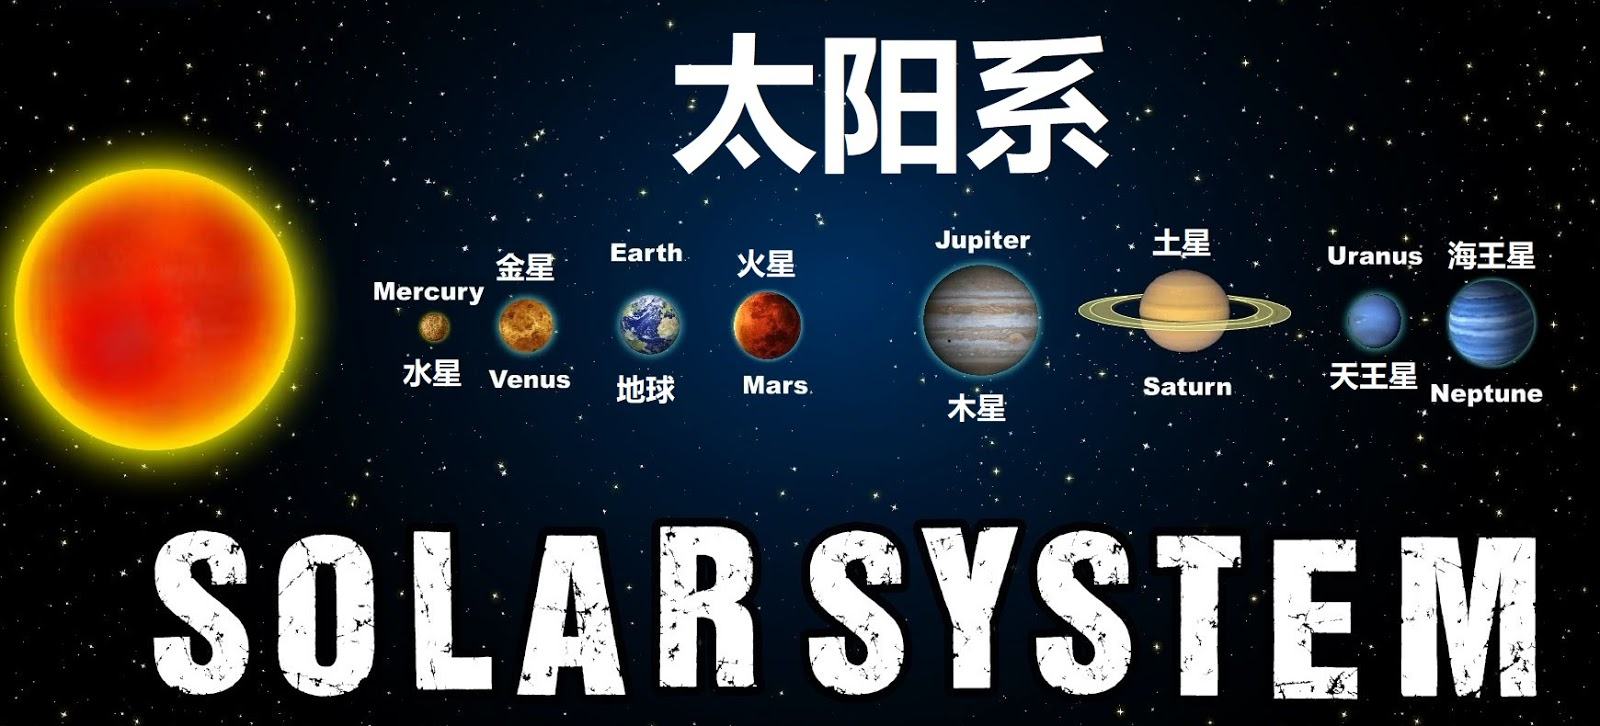
\includegraphics[width=0.5\linewidth]{images/太阳系.jpg}
    \caption{太阳系图片展示}
    \label{fig:solar system}
\end{figure}

本研究的创新性体现在两方面:其一,通过引入四阶龙格-库塔方法处理四体问题,突破了传统三体模型的局限性;其二,在判别条件设计中,我们严格依据国际天文联合会(IAU)的日月食判据标准,并针对数值计算结果开发了自动化事件检测算法。最终实现的预测结果与NASA权威星历表的高度吻合,不仅验证了模型的有效性,更彰显了数学建模在现代天体力学研究中的核心价值。

\section{理论分析}
\subsection{总论}
经典的$N$体运动方程为:
$$
M_i\ddot{\mathbf{r}}_i = \sum_{j=1}^N\frac{GM_iM_j}{||\mathbf{r}_j-\mathbf{r}_i||^3}(\mathbf{r}_j-\mathbf{r}_i)
$$
其中${M_i}$为各个天体的质量,$\mathbf{r}_i$为各个天体的位矢。
在模拟太阳系的过程中,完整的牛顿运动方程就应该是包含所有天体及其相互作用的N体运动。
\subsection{A Toy Model}
仅考虑三体运动,日地月系统的运动方程为:
\begin{align*}
    M_s\ddot{\mathbf{r}}_s&=\frac{GM_sM_e}{||\mathbf{r}_e||^3}\mathbf{r}_e+\frac{GM_sM_m}{||\mathbf{r}_m||^3}\mathbf{r}_m\\
    M_e\ddot{\mathbf{r}}_e&=-\frac{GM_sM_e}{||\mathbf{r}_e||^3}\mathbf{r}_e+\frac{GM_mM_e}{||\mathbf{r}_m-\mathbf{r}_e||^3}(\mathbf{r}_m-\mathbf{r}_e)\\
    M_m\ddot{\mathbf{r}}_m&=-\frac{GM_sM_m}{||\mathbf{r}_m||^3}\mathbf{r}_m+\frac{GM_eM_m}{||\mathbf{r}_e-\mathbf{r}_m||^3}(\mathbf{r}_e-\mathbf{r}_m)
\end{align*}
\subsection{误差及修正分析}
本节中对常见的需要纳入考量的影响因素的误差及其处理方式做了讨论。
\subsubsection{理论误差}
这里主要讨论了使用的物理理论并非精确带来的误差。
\paragraph{相对论}
狭义及广义相对论直接改变了最底层运动方程,其带来的影响无法严格计算,但影响的量级可以估计为 $\epsilon_r=(\frac{v}{c})^2\sim(\frac{2\pi r_e}{cT_e})^2\sim1\times10^{-8}$。
\\
\\
相对论(尤其是广义相对论)的引入会极大地增加求解的难度和复杂度,在这里不得不将其忽略,因此所得结果的误差界量级至少也有$10^{-8}$,此后所有影响量级在此之下的误差均会在讨论中指出并直接忽略。
\subsubsection{对象误差}
这里主要讨论了讨论的日地月系统外的天体系统及其效应带来的误差。
\paragraph{大行星和惯性力}
以木星为代表的大行星质量相对大,与地球距离相对近,其产生的引力扰动量级可以估计为$\epsilon_j\sim\frac{M_jr_e^2}{M_s(r_j-r_e)^2}\sim5\times10^{-5}$。
同时,太阳受到太阳系内各个行星的作用导致以太阳作为参考系时天体受到惯性力的作用,其产生的扰动量级可以估计为$\epsilon_a\sim\frac{M_jr_e^2}{M_sr_j^2}\sim4\times10^{-5}$,这个扰动与大行星的扰动同源,必须同时忽略或纳入考虑。
\paragraph{银河系以及更大的天体系统}
太阳系以约2.2亿个地球年为周期绕银河系作半径约为2.6万光年公转,同时银河系的其他部分的引力也会对太阳系中的天体产生长程作用,这个作用的强度可利用潮汐效应来估计$\epsilon_g\sim(\frac{2\pi}{T_s})^2r_s\frac{r_e}{r_{nearest}}\sim8\times10^{-16}$,可以直接忽略。
\\
\\
为处理大行星和惯性力带来的影响,除了直接将大行星加入天体系统进行模拟,也可以采用渐进微扰的思路。
将各个系统绕太阳作独立圆周运动作为零阶微扰的结果,各个系统间的影响视作一阶效应,由于二阶及更高的效应量级为$\epsilon^2\sim10^{-10}$可以忽略,我们最终求解的系统就是一个独立系统加上其他部分对其一阶微扰的结果。
处理一个N体问题的复杂度为$O(N^2)$,而将大行星的影响以微扰的形式加入的计算复杂度为$O(N)$。
因此当$N$足够大时,这个方案能极大的简化模拟,然而在实际应用中发现唯二对系统产生有效影响的行星只有木星和金星,在这个系统尺度下微扰的方法并没有优势。
\subsubsection{几何误差}
这里主要讨论将天体建模为质点带来的引力计算上的误差。
\paragraph{非球形建模}众所周知由于自转效应的影响地球是一个两极稍扁赤道略鼓的椭球,这就导致地球的引力并非严格等效于球心处的质点,考虑引力场的的球谐展开:
\begin{align*}
    G(\mathbf{r})&=\int_{\Omega}\frac{G\rho(\mathbf{R})}{||\mathbf{R}-\mathbf{r}||}\mathrm{d}^3\mathbf{R}\\
    &=G\sum_{n=0}^\infty\frac{1}{r^{n+1}}\int_\Omega R^n\rho(\mathbf{R})P_n(\cos{\psi})\mathrm{d}^3\mathbf{R}
\end{align*}
其中$P_n$为$n$阶勒让德多项式。
可见高阶矩的影响随着距离的增加而迅速减弱(以地月系统为例$\frac{||\mathbf{R}_e||}{||\mathbf{r}_m-\mathbf{r}_e||}\sim0.02$),实验测量给出地球二阶系数的量级$J_2\sim1\times10^{-3}$,因此唯一可能有有效影响的$J_2$摄动在地月系统中影响量级为$\epsilon_e\sim(\frac{||\mathbf{R}_e||}{||\mathbf{r}_m-\mathbf{r}_e||})^2J_2\sim4\times10^{-7}$,而与太阳相关的摄动影响更加不明显,无需纳入考虑。

\subsubsection{观测误差}
由于我们预测的是“观测到日(月)食的时间”,所以一些观测建模上的误差也要纳入讨论。
\paragraph{光传播用时}
在宇宙尺度中光速会让日(月)食的发生不再是一个单纯的几何问题,由于发生时日地月基本在一条直线上,月(地)对太阳光线的遮挡与地球上观测到这个现象之间间隔的时间可以直接用光传播的时间进行近似$\Delta t_l\sim2\frac{||\mathbf{r}_e-\mathbf{r}_m||}{c}\sim2s$,发生和观测时间的不同步也会对日(月)食判断的几何条件带来影响,这个影响带来的时间上的误差也在同一量级。
\paragraph{大气}
标准大气的折射率$n_a=1+2.9\times10^{-4}$,在地球大气层随着高度的上升,这个值由于空气变得稀薄越来越接近于1,这会导致光线产生弯曲。另外,光的散射也会导致部分波长的光到达月球后强度有不同程度的减弱,从而带来其他观测上的效应。对于日食,这个偏转作用在地球表面量级为$\theta=\theta_0-\sin^{-1}(\frac{1}{n_a}\sin\theta_0)\sim1.4^\circ$,对时间的影响量级为$\Delta t_n\sim\frac{\theta}{2\pi}T_0\sim20s$,但是这个误差随一天不同时间的变化明显,在接近日出(日落)时最为明显,在正午则无理论影响。对于月食,这个误差等效为地球半径的变化(即大气层的一部分由于光的被散射或是吸收从而增大了地球的阴影范围),但因为大气密度随着海拔指数的下降,在距离地表50km处就下降到地表处的1\%以下,大气对地球有效半径的影响甚至没有地球本身形状带来的影响明显。
\paragraph{其他几何因素}
地月半径的不均匀等其他几何因素也会对日(月)食的形态产生影响,但不会显式的影响到日(月)食发生的客观时间。
\\
\\
这一部分出现的误差由于直接作用于观测端,并不能直接与前面提到的建模误差进行量级上的比较。可以根据最后误差的敏感性来考量是否将其纳入考虑。
\subsubsection{结论}
按照前面提出的处理方法,最终观测时间的误差阶为$4\times10^{-7}\pm20s$。
在50年的尺度下看,也就是$\pm50 y.\times 4\times10^{-7}\pm20 s\sim \pm10min$。
以上分析均为理论估计,具体的影响量级需要在之后的实验中做进一步验证。
\subsection{运动方程的无量纲化处理}
为了避免大量的不同量级常数运算,在数值模拟过程中对所有运动方程做了无量纲化处理。
具体为:
\begin{align*}
    \tilde{t}&=\frac{t}{3600s/h}\\
    \tilde{r}&=\frac{r}{1.495979\times10^8km/a.u.}
\end{align*}
同时修改质量的量纲,使得万有引力常数$G=1$。

\vspace{10pt}


以下,我们将讨论如何判定日食与月食:

\subsection{日食判定}
\subsubsection{定义与符号说明}
\begin{figure}[H]
    \centering
    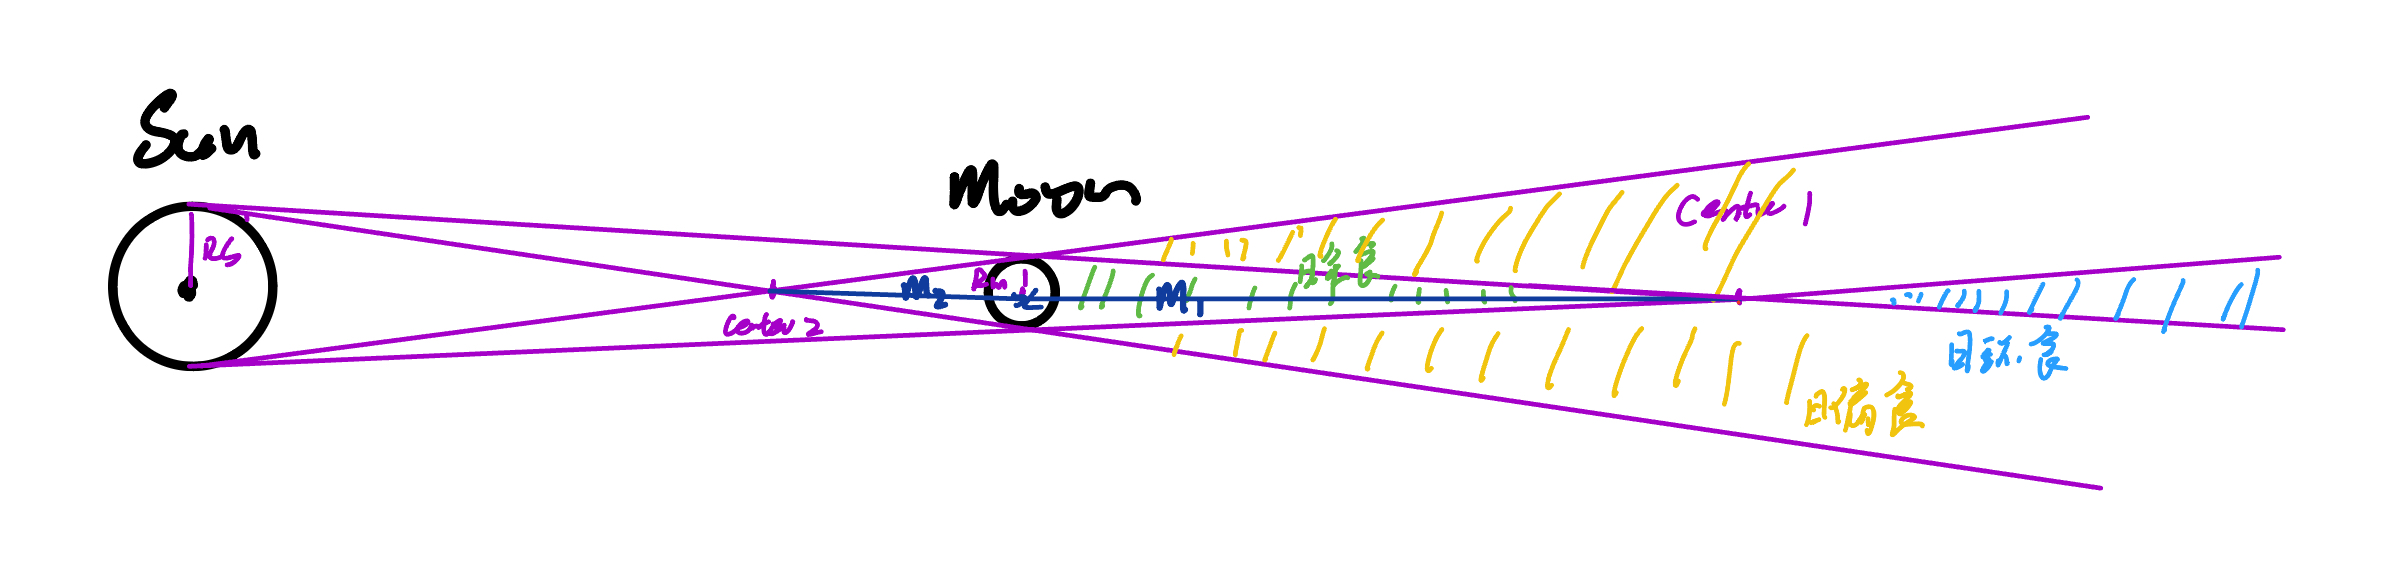
\includegraphics[width=0.8\linewidth]{images/sun_moon_pos.jpg}
    \caption{太阳 - 月球位置关系图}
    \label{fig:sun_moon_rela}
\end{figure}

如图\ref{fig:sun_moon_rela}所示,地球上某点在绿色、蓝色和黄色阴影处分别对应其将观察到日全食、日环食和日偏食。我们已经有太阳、月球中心的位置,不妨设太阳中心为$S$点(原点),月球中心是$M$。本影锥、半影锥的顶点分别设为$C_1,\ C_2$。记$\mathbf{m_1} = \overrightarrow{C_1M},\ \mathbf{m_2} = \overrightarrow{C_2M}$. 另记本影(umbra)的集合(绿色阴影区域)为$U$,半影(penumbra)的区域(黄色阴影)为$P$,伪本影(antumbra)的区域(蓝色阴影)为$A$. 

\begin{figure}[H]
    \centering
    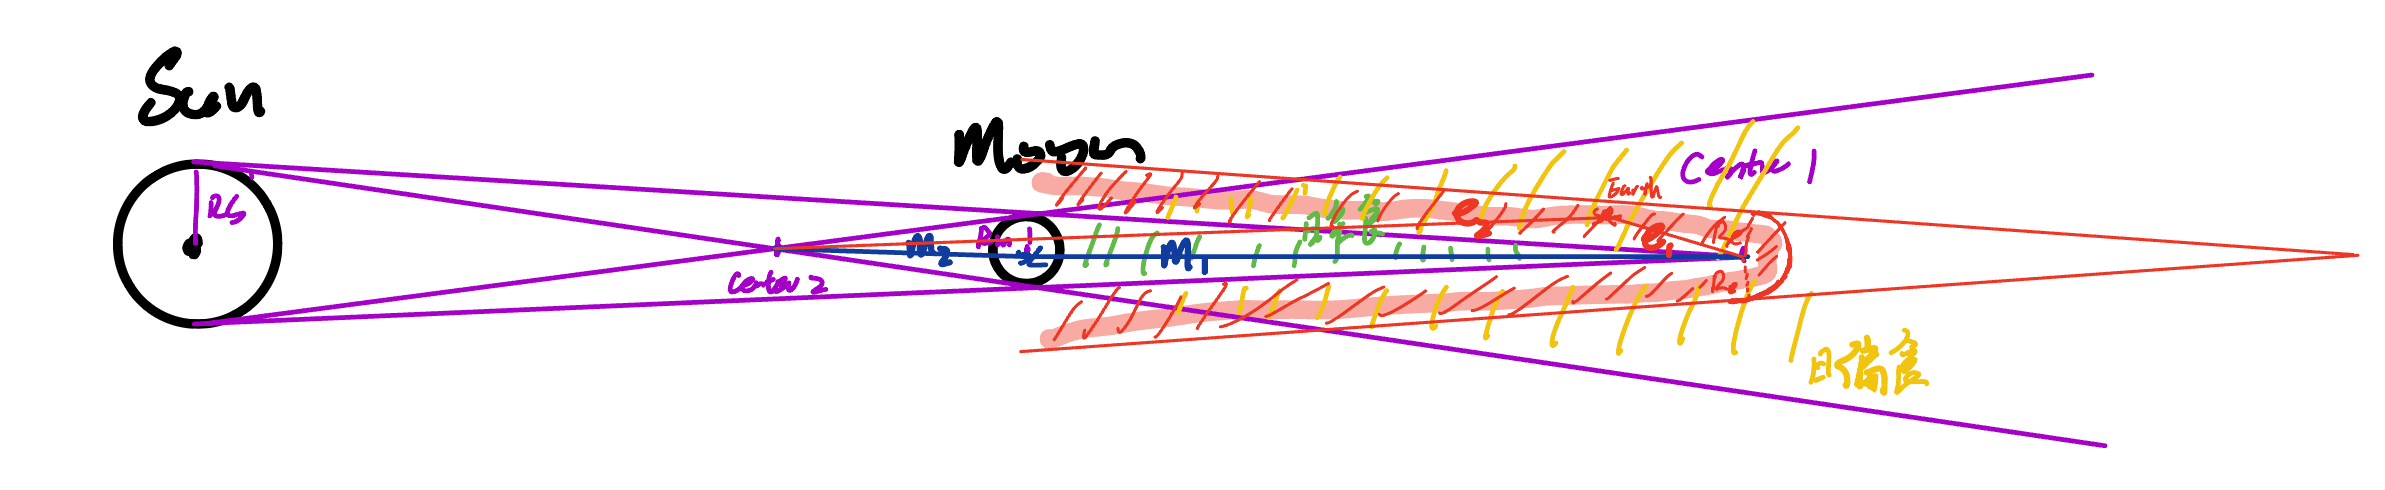
\includegraphics[width=0.8\linewidth]{images/image.png}
    \caption{日全食的判定示意图}
    \label{fig:total_eclipse_deter}
\end{figure}

现在我们加入地球的中心E,记$\mathbf{e_1} = \overrightarrow{C_1E},\ \mathbf{e_2} = \overrightarrow{C_2 E}$. 经过几何观察,容易发现当地球球心$E$处于$T = \{x| d(x, U) < R_e\}$时(图\ref{fig:total_eclipse_deter}示红色区域),地球上会有点陷入日全食,我们认为这时地球上发生的日食就是日全食。


\begin{figure}[H]
    \centering
    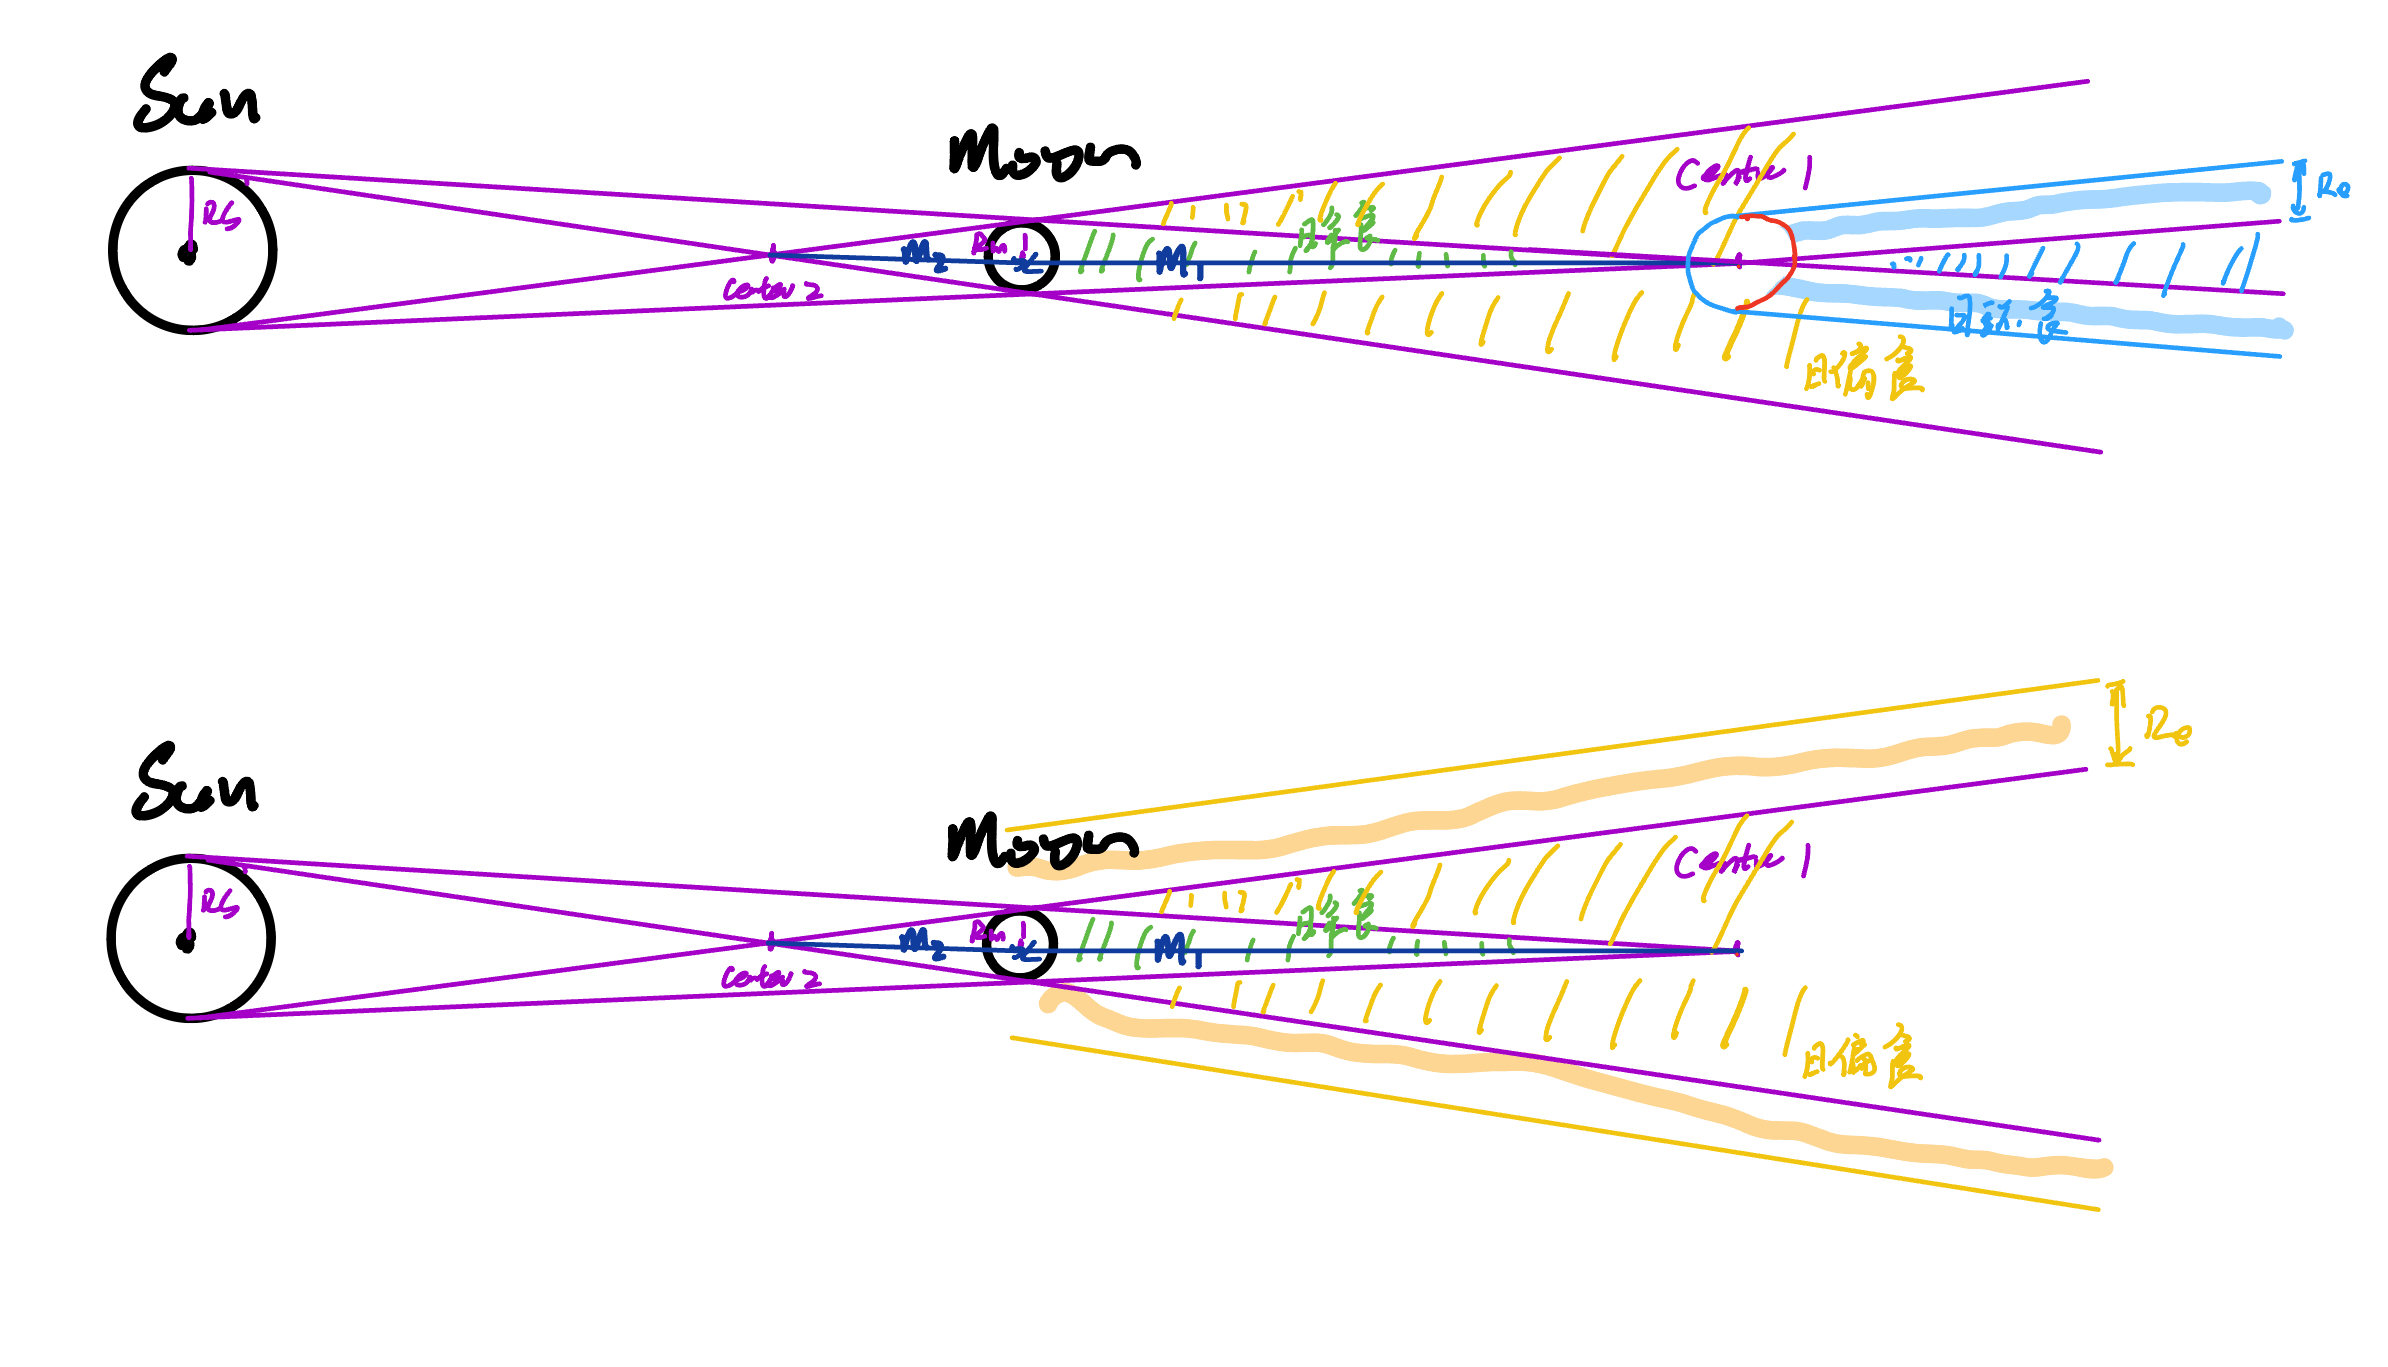
\includegraphics[width=0.8\linewidth]{images/annular_partial_eclipse.jpg}
    \caption{日环食、日偏食判定示意图}
    \label{fig:enter-label}
\end{figure}

当地球球心$E$距离伪本影区域的距离小于$R_e$、且不在$T$内时($Ann = \{x | d(x, A)<R_e\} - T$),地球上有区域发生了日环食,我们认为这时地球上发生的日食是日环食。

最后,当地球球心距离半影锥小于$R_e$,且不在$T\cup Ann$内($Par = \{x| d(x, P) < R_e\}\ -\ T\cup Ann$),我们认为地球上发生了日偏食。

\subsubsection{Thresholds与判定条件推导}

\begin{figure}[H]
    \centering
    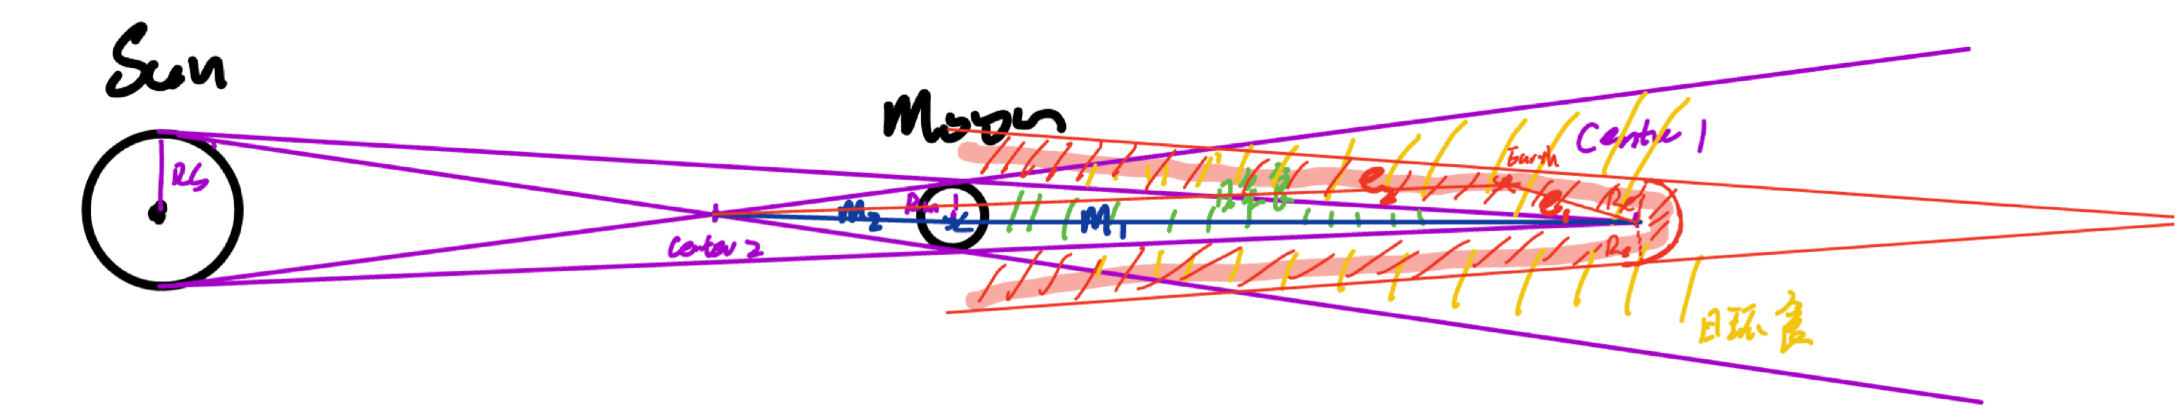
\includegraphics[width=0.8\linewidth]{images/total_eclipse.jpg}
    \caption{日全食条件推导}
    \label{fig:enter-label}
\end{figure}

如图,设红色阴影区域的边界可以延申至O点,那么$\dps\overrightarrow{OE} = \frac{R_e}{R_m}\mathbf{m_1} + \mathbf{e_1}$. 

我们记本影锥向外拓展$R_e$所扩成的新锥体为$C$,于是
\begin{align}
E\in C & \Longleftrightarrow \sin\langle \overrightarrow{OE}, \mathbf{m_1}\rangle < \sin \theta = \frac{R_m}{\|\mathbf{m_1}\|}\\
& \Longleftrightarrow \frac{\| (\frac{R_e}{R_m}\mathbf{m_1} + \mathbf{e_1})\times \mathbf{m_1}\|}{\|\frac{R_e}{R_m}\mathbf{m_1} + \mathbf{e_1}\| \|\mathbf{m_1}\|} < \frac{R_m}{\|\mathbf{m_1}\|}\\
& \Longleftrightarrow \| \vt{e_1} \times \vt{m_1}\| < \norm{R_e\vt{m_1} + R_m\vt{e_1}}\\
& \Longleftrightarrow T_1 
 := \norm{\vt{e_1} \times \vt{m_1}}^2 - (R_e^2 \norm{\vt{m_1}}^2 + R_m^2 \norm{\vt{e_1}}^2 + 2R_e R_m \vt{m_1}\cdot \vt{e_1}) < 0
\end{align}

$T_1$即为我们的第一个threshold,我们注意到$T_1 < 0$不一定代表日食发生。而在交入$d_1 = \vt{e_1} \cdot\vt{m_1} > 0$和
$d_0 = \overrightarrow{ME}\cdot \overrightarrow{SE} >0$
这两个条件后,所得到的区域$\Omega_1$一定可以观测到日全食。又注意到当$E\in \Omega_2 = \{E\ | \norm{\vt{e_1}} < R_e\}$时,也一定有日全食发生。我们可以近似认为$\Omega_1 \cup \Omega_2$就是整个红色+绿色阴影区。

\begin{figure}[H]
    \centering
    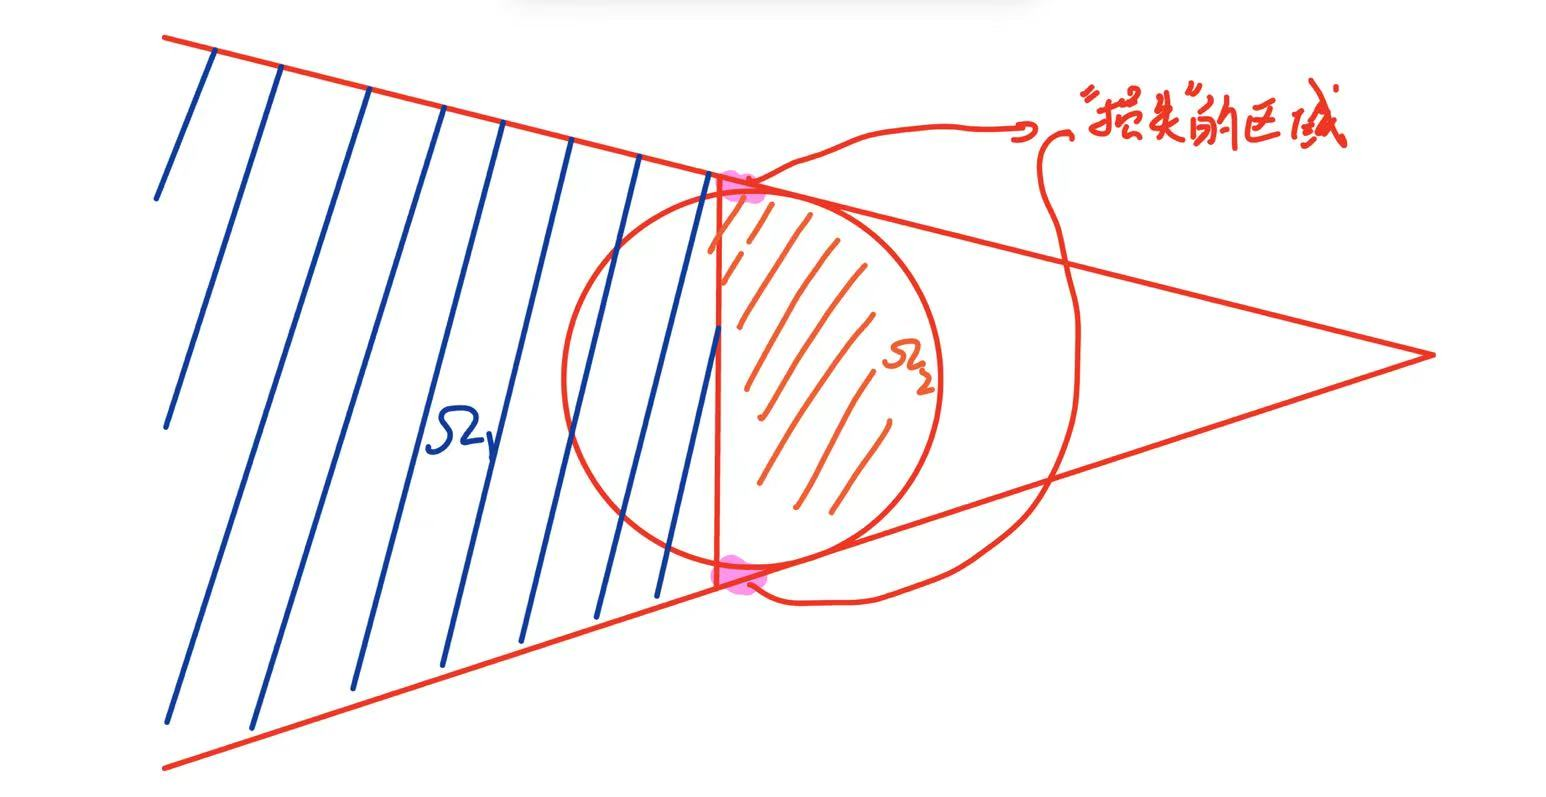
\includegraphics[width=0.5\linewidth]{images/lost_regions.jpg}
    \caption{损失的区域}
    \label{fig:enter-label}
\end{figure}
事实上,这样做我们可能会丢失一些区域(见图5),也就是锥面与球面尚未相切的部分区域,然而由于锥顶角$\theta$极小($\dps\sim \frac{R_m}{\norm{ME}} = 4.5\times10^{-3}$)故可以忽略。

小结:在这一部分,布尔条件$b_1 = (T_1 < 0 \mbox{ and } d_1 > 0 \mbox{ and } d_0 > 0)\ \mbox{ or } (\norm{\vt{e_1}} < R_e)$若$==1$,则日全食发生。

\begin{figure}
    \centering
    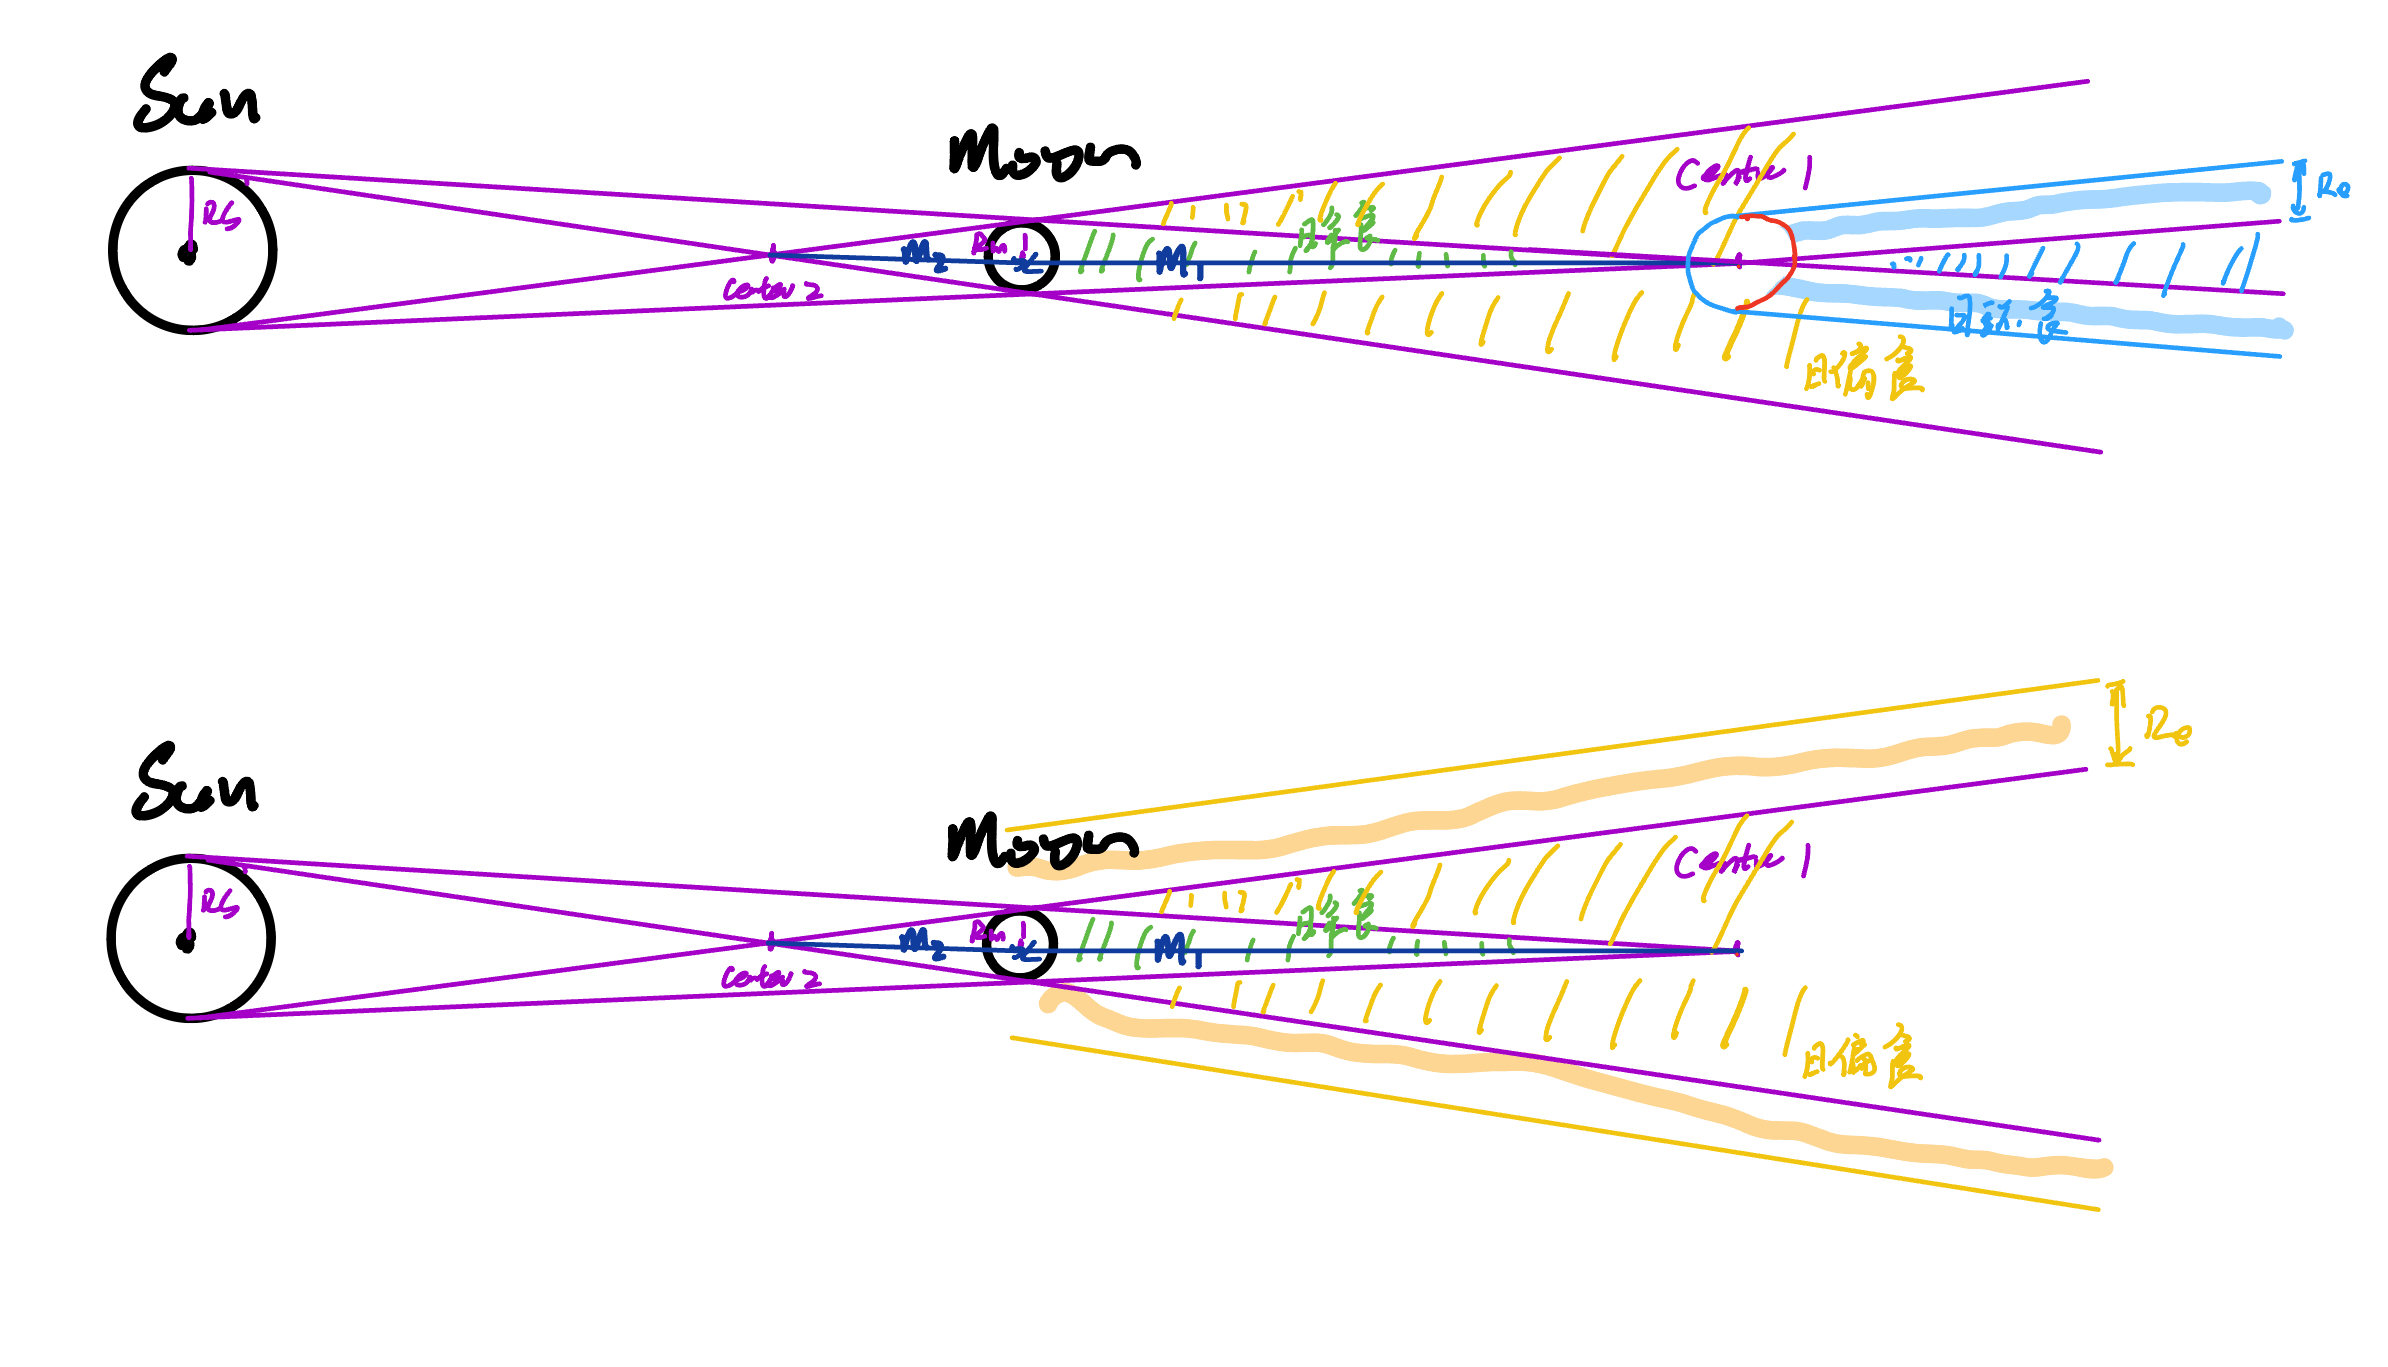
\includegraphics[width=0.8\linewidth]{images/annular_partial_eclipse.jpg}
    \caption{日环食、日偏食地球中心的所在区域}
    \label{fig:enter-label}
\end{figure}

我们可以类似地推导日环食与日偏食的发生条件,得到thresholds $T_3, T_2$(分别对应环食/偏食)和布尔条件(thresholds 推导见附录)
$$
T_3
 := \norm{\vt{e_1} \times \vt{m_1}}^2 - (R_e^2 \norm{\vt{m_1}}^2 + R_m^2 \norm{\vt{e_1}}^2 - 2R_e R_m \vt{m_1}\cdot \vt{e_1})
$$
$$
T_2 := \norm{\vt{e_2} \times \vt{m_2}}^2 - (R_e^2 \norm{\vt{m_2}}^2 + R_m^2 \norm{\vt{e_2}}^2 + 2R_e R_m \vt{m_2}\cdot \vt{e_2}) < 0
$$
$$
b_2 = (\mbox{ not } b_1) \andd ((T_3 < 0) \andd (d_1 \leq 0) \andd (d_0 > 0)),\quad b_2 == 1 \Longleftrightarrow \text{日环食发生}
$$ $$
b_3 = (\nott b_1) \andd (\nott b_2) \andd (T_2 < 0) \andd (d_0 > 0), \quad b_3 == 1 \Longleftrightarrow \text{日偏食发生}
$$


\subsection{月食判定}

月食的判定与日食的判定没有本质区别,但是由于太阳 - 地球形成的本影锥顶点(即$C_1$)到地球的距离远大于地月距离,前者的距离是$\dps \norm{SE}\frac{R_e}{R_s - R_e} \approx 1.38\times 10^9$米,而后者只有约$3.8\times 10^8$米。因此,针对月球我们只需考虑全食和偏食的情形。甚至,针对月球中心在$C_1$点附近的精细分析也因为上面提到的距离差而毫无必要。

需要注意的是,月偏食的定义为月球的一部分进入地球的本影,月全食的定义是月球的全体进入本影,这点需要与日偏食/日全食的定义区分开。

通过迁移日食的推导,我们给出月食的thresholds和判定月食的条件:
$$
T_4 
 := \norm{\vt{m_1} \times \vt{e_1}}^2 - (R_m^2 \norm{\vt{e_1}}^2 + R_e^2 \norm{\vt{m_1}}^2 + 2R_e R_m \vt{m_1}\cdot \vt{e_1}) < 0
$$
$$
T_5 
 := \norm{\vt{m_1} \times \vt{e_1}}^2 - (R_m^2 \norm{\vt{e_1}}^2 + R_e^2 \norm{\vt{m_1}}^2 - 2R_e R_m \vt{m_1}\cdot \vt{e_1}) < 0
$$
$$
b_4 = (T_4 < 0) \andd (\vt{m_1} \cdot \vt{e_1} > 0) \andd (d_0 > 0), b_4 == 1 \Longleftrightarrow \text{月全食发生}
$$
$$
b_5 = (T_4 < 0) \andd (T_5 > 0) \andd (d_0 > 0), b_5 == 1 \Longleftrightarrow \text{月偏食发生}
$$

\begin{figure}
    \centering
    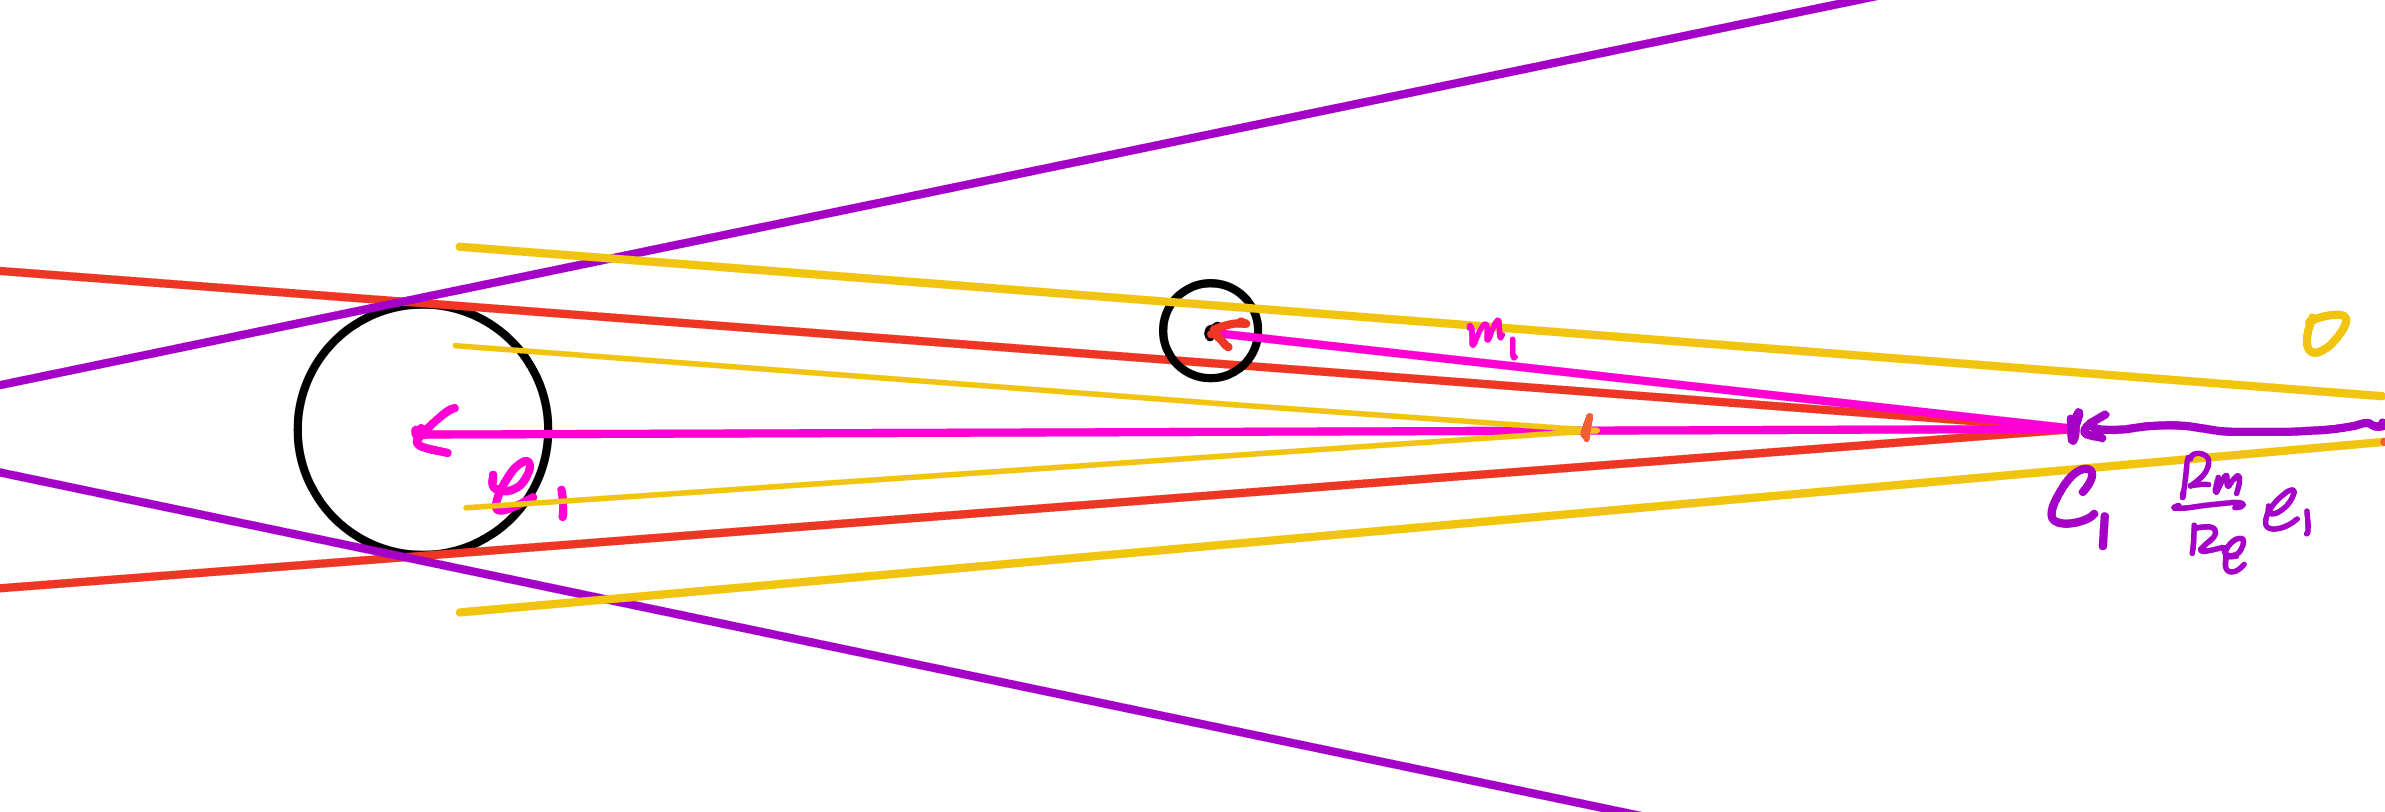
\includegraphics[width=0.8\linewidth]{images/moon_eclipse.png}
    \caption{月球中心进入外侧黄V字形代表月偏食开始,进入内侧黄V字形代表全食开始}
    \label{fig:enter-label}
\end{figure}

\subsection{实现代码:\text{check\_eclipse.py}}


\section{数值算法分析}

为了判定日食与月食,我们构建起三维立体网络,运用牛顿万有引力定律进行模拟。在上一节中,我们分析了常见的误差项,并给出了判定日月食的方法。在本节中,我们将讨论如何对这个三体系统进行数值模拟,并对优化效率进行探讨。

\subsection{Runge - Kutta 方法}

本项目主要使用四级四阶古典显式Runge - Kutta方法进行估计。
\subsubsection{方法介绍}

四级四阶古典显式Runge - Kutta方法由以下公式给出:

\begin{align*}
y_{n+1} &= y_n + \frac{h}{6} \left(k_1 + 2k_2 + 2k_3 + k_4\right)\\
k_1 &= f(t_n, y_n) \\
k_2 &= f\left(t_n + \frac{h}{2},\; y_n + \frac{h}{2}k_1\right) \\
k_3 &= f\left(t_n + \frac{h}{2},\; y_n + \frac{h}{2}k_2\right) \\
k_4 &= f\left(t_n + h,\; y_n + h k_3\right)
\end{align*}

本例中,我们令$\vt{y} = (\vt{r_s}, \dot{\vt{r_s}}, \vt{r_e}, \dot{\vt{r_e}}, \vt{r_m}, \dot{\vt{r_m}})^T$, 则
\begin{align*}
\dot{\vt{y}} &= (\vt{r_s}, \dot{\vt{r_s}}, \vt{r_e}, \dot{\vt{r_e}}, \vt{r_m}, \dot{\vt{r_m}})^T = (\dot{\vt{r_s}}, \vt{F_s}(\vt{r_s}, \vt{r_e}, \vt{r_m}), \dot{\vt{r_e}}, \vt{F_e}(\vt{r_s}, \vt{r_e}, \vt{r_m}), \dot{\vt{r_m}}, \vt{F_m}(\vt{r_s}, \vt{r_e}, \vt{r_m}))^T\\
&= f(\vt{y})
\end{align*}
步长$h = 1 \mbox{ hour}$,这里$F_s, F_e, F_m$的表达式由2.2章给出。

\subsubsection{数值稳定性分析}

我们计算初始的Jacobi矩阵来验证:
\[
J = \frac{\partial F(y)}{\partial y} =
\begin{bmatrix}
0 & I & 0 & 0 & 0 & 0 \\
A_{11} & 0 & A_{12} & 0 & A_{13} & 0 \\
0 & 0 & 0 & I & 0 & 0 \\
A_{21} & 0 & A_{22} & 0 & A_{23} & 0 \\
0 & 0 & 0 & 0 & 0 & I \\
A_{31} & 0 & A_{32} & 0 & A_{33} & 0
\end{bmatrix}
\]

其中,对于$i \neq j$, \( A_{ij} = \frac{\partial \vec{a}_i}{\partial \vec{r}_j} \) 是加速度对位置的偏导数。具体地,雅可比矩阵的各个块表示为:

\[
A_{ij} = G m_j \left( \frac{I}{r^3} - 3 \cdot \frac{\vec{r} \vec{r}^T}{r^5} \right)
\]
其中 \( r = \vec{r}_j - \vec{r}_i \) 是位置向量,\( r \) 是两物体之间的距离,\( I \) 是单位矩阵,\( G \) 是万有引力常数,\( m_j \) 是天体的质量。
\\
对于$i = j$, $\dps A_{ii} = - \sum_{k\neq i}A_{ik}$.

代码实现:jacobi.py, 按月计算发现最大的最大值模$\lambda_{ultra} = \max_{1\le t\le 600}\{\lambda_{max, t}\} = 0.0152$. 于是,
$$\frac{\partial \phi(t_n, y_n, h)}{\partial y_n} = \frac 1 6(k_1 + 2k_2 + 2k_3 + k_4) \le \lambda_{ultra}$$,全局误差$GTE \sim O((h\lambda)^4)$,后者大约在$10^{-7}$量级,因此可以感受到其稳定性是足够的(没学过数值分析完全不知道怎么说,只能照猫画虎一下,请老师见谅)。如图所示,$\lambda_t$一直稳定地保持在低位震荡。
\begin{figure}[h]
    \centering
    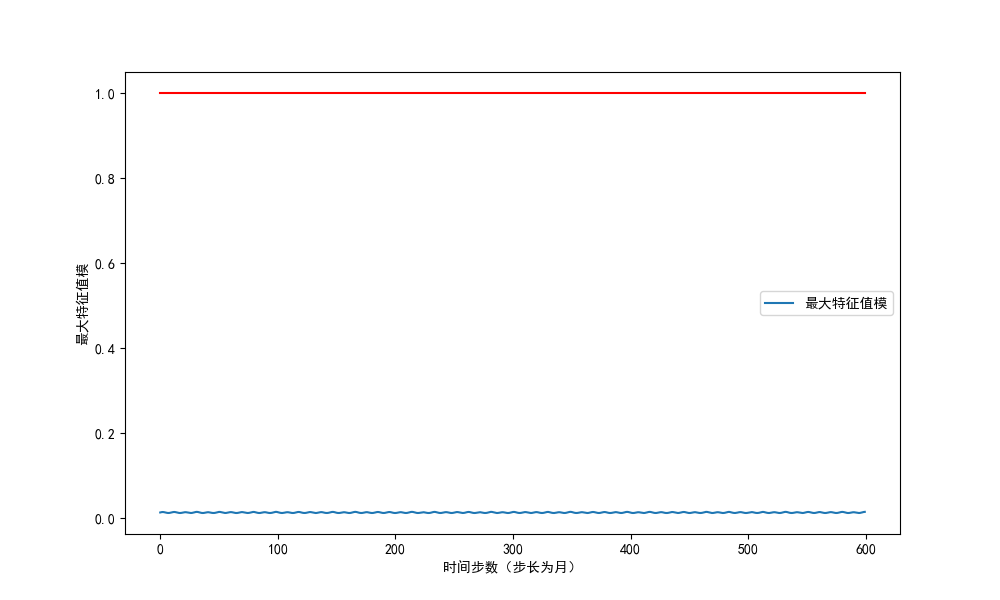
\includegraphics[width=0.8\linewidth]{images/Figure_12.png}
    \caption{最大特征值模的稳定性}
    \label{fig:enter-label}
\end{figure}

\subsection{时间判定与日食转换}

\subsubsection{时间判定}


日食、月食是概率罕见的天文事件,可能几年一遇,如果采用精细时间步长计算,会造成大量算力浪费,所耗时间显著提高。如果以大步长计算,模型的收敛性可能无法保证(参见test\_heun\_trajectory\_v1(1).ipynb),而且可能会跳过一些较短时长的日食或者月食。

我们采用以下的方式:先用coarse\_step = 1小时 来逐步模拟,这是一个不短不长的时间步长,能够保证探测到绝大多数日食/月食;然后,如果探测到日食/月食,在日月食开始/结束的边界位置用$\dps\frac{1}{fine\_steps} = \frac 1 {100}$小时的宽度进行模拟,找出日食/月食的精确开始/结束时间。

\subsubsection{日月食转换}
任何的日全食、日环食,都在开始后和结束前的一小段时间内为日偏食。这个阶段,地球尚未运动到(或已经移出)本影/伪本影所在区域,但已经身处半影中。因此,程序会先探测到日偏食,再探测到日全食或者日环食。因此,如果我们不做任何处理,程序会输出同一个日期多个日食的情况,这是不合情理的。

为此,我们向前和向后检测日偏食周围两个小时的事件,如果检测到日全食或者环食,就跳过当前事件。

月食的处理同日食一致。

\subsection{全环食问题}

在日食转换的过程当中,比较常见的有日偏食向日全食/日环食转换,或者反之。但是,我们进一步发现有一类新的日食——全环食,可能出现日全食/日环食相互转换的情况。
\begin{figure}[h]
    \centering
    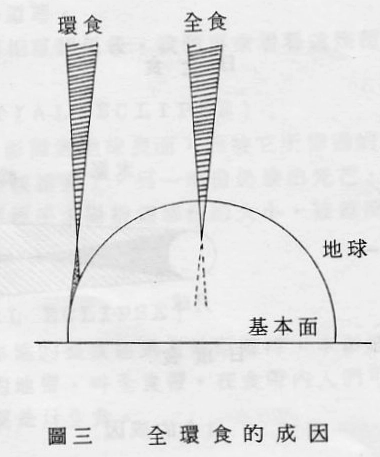
\includegraphics[width=0.4\linewidth]{images/hybrid_eclipse.png}
    \caption{全环食的成因}
    \label{fig:hybrid_eclipse}
\end{figure}

全环食的成因如\ref{fig:hybrid_eclipse}
所示,月球的运动使得本影锥的顶点轨迹正好穿过地球,形成部分全食、部分环食的景象。在NASA的数据库中,这类日食被标记为日环食;在我们的初始模拟中,这类日食被标记为日全食。它们的存在给我们带来了不少困扰,直到我们发现这两种说法各有对的一面。在本项目中,我们把全环食记成日全食。

\section{实验结果}

目前根据我们的数值算法,已实现对2025年至2075年全部日食和月食事件的百分百预测。此部分中所有实验选取同一个对照组,采用的参数是:模拟日地月木金的体系,时间步长取为1小时。
如此得到的预测结果中,对食分时刻的预测误差控制在20min以内,极少事件会出现10min以上的误差(见图\ref{fig:eclipse_error}),这和理论误差分析的结果在量级上吻合的很好。

\begin{figure}[h]
    \centering
    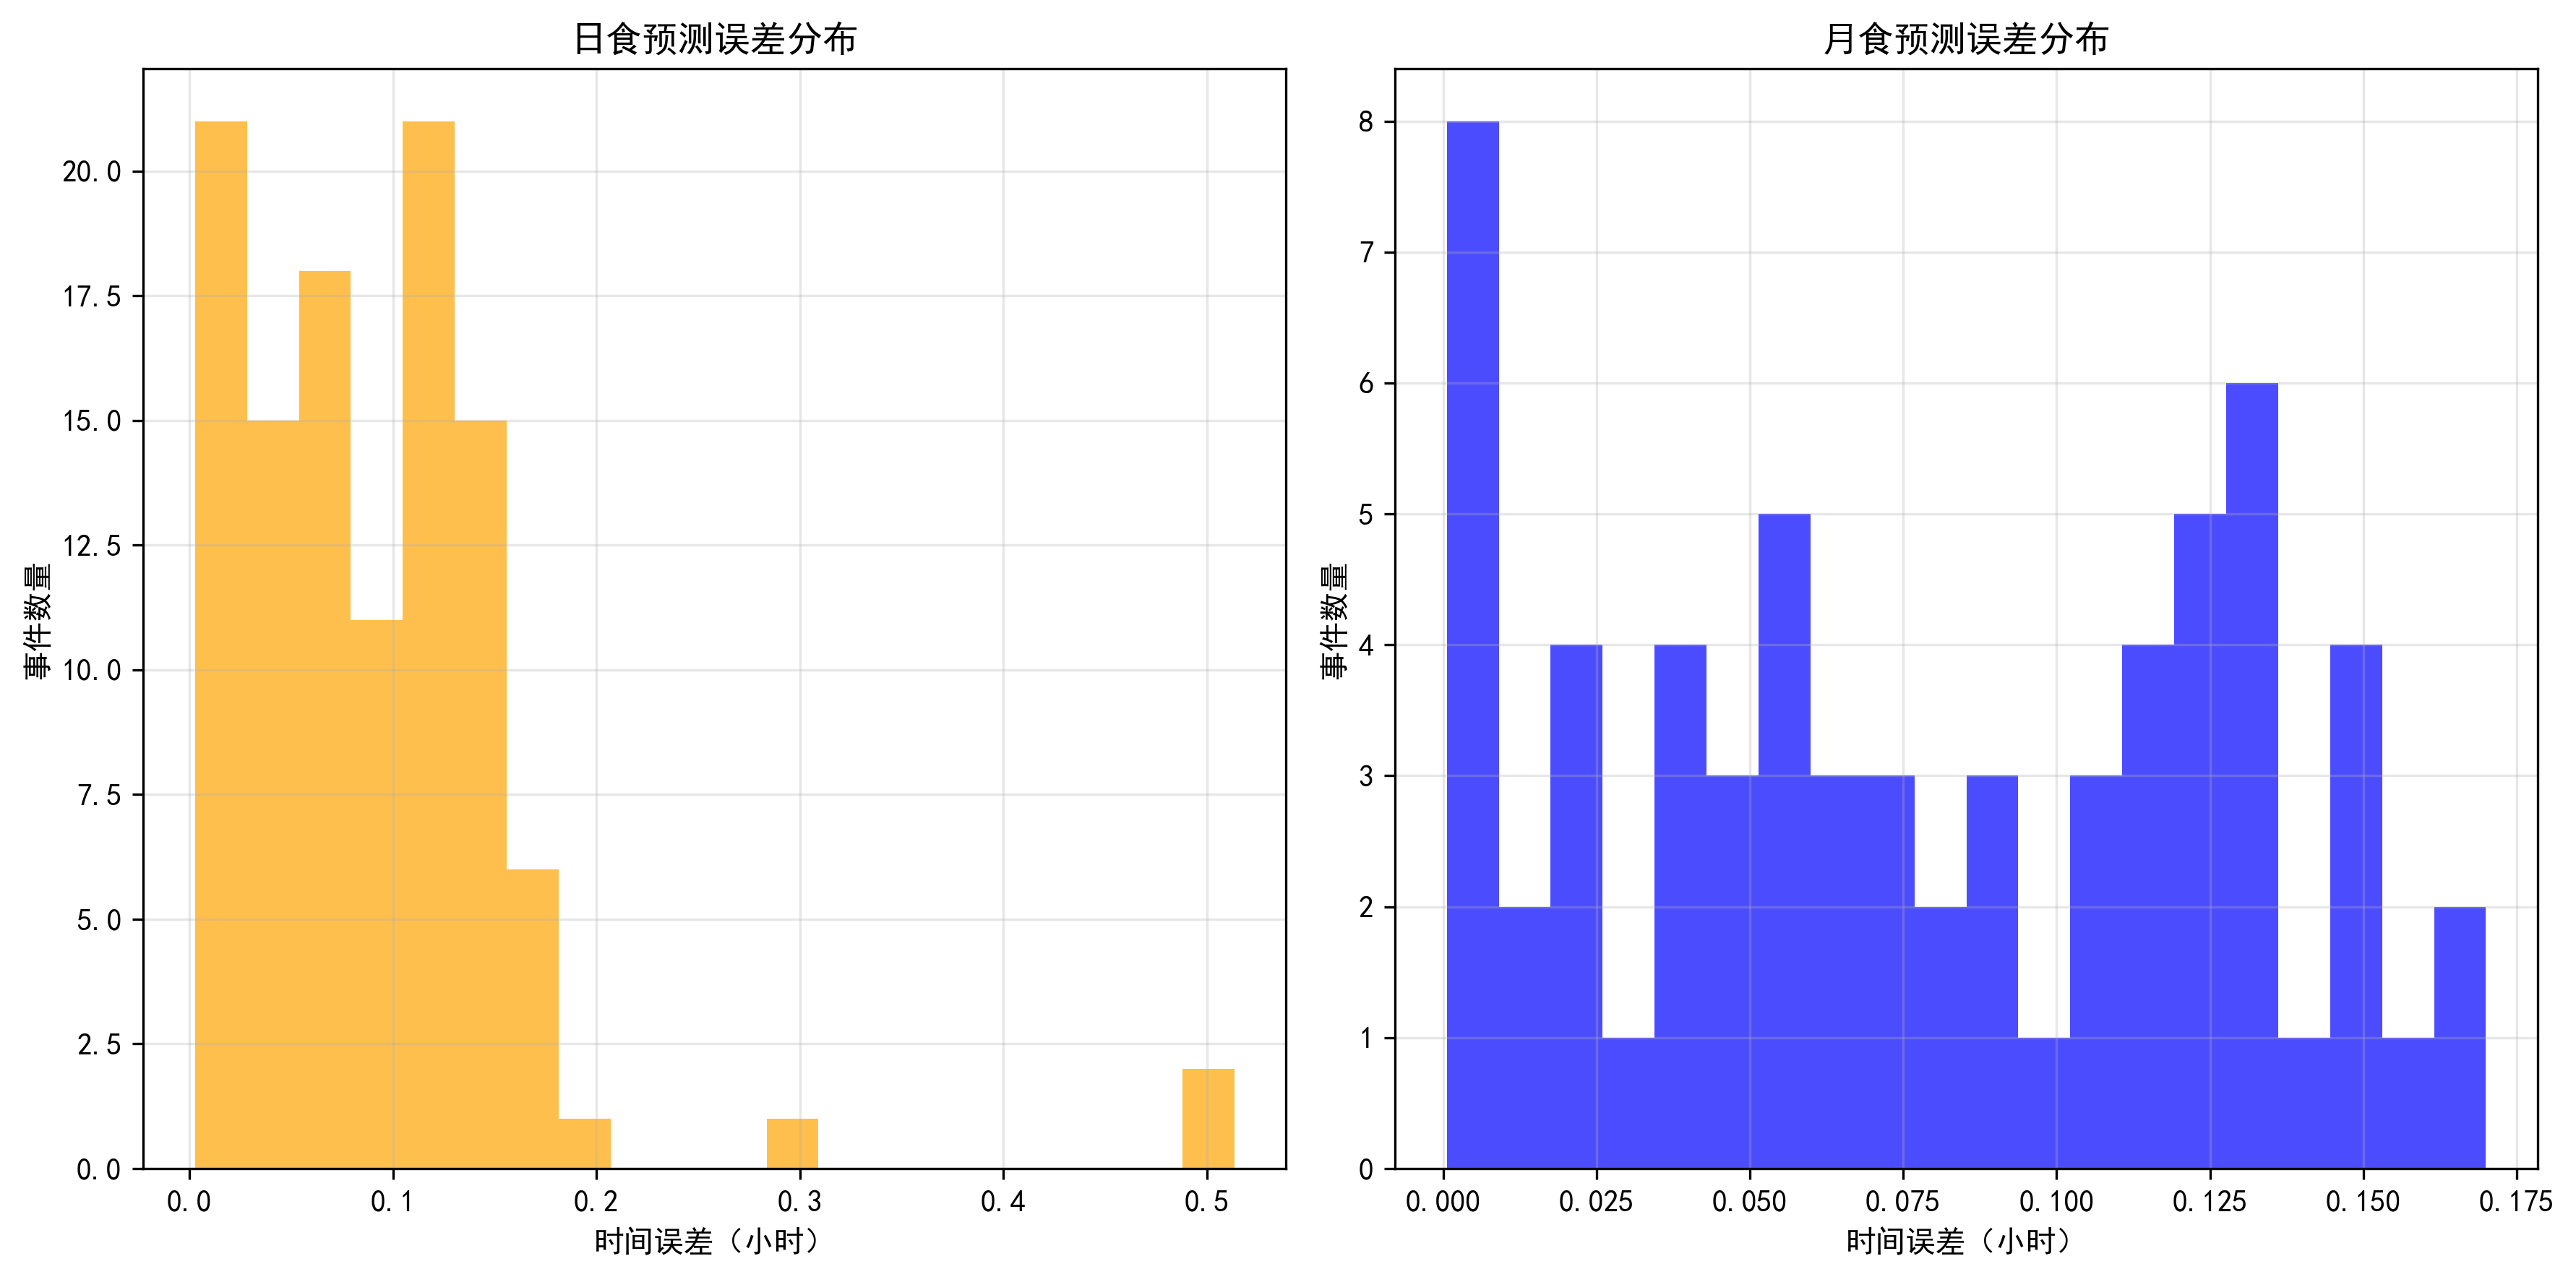
\includegraphics[width=0.5\linewidth]{images/error_distribution_1.png}
    \caption{对照组(预测准确率96.70\%)}
    \label{fig:eclipse_error}
\end{figure}

同时绘制了此对照组对应的地月位置和星表中标准值的误差变化曲线,如图\ref{fig:position_error}所示(图中的负号由于绘图原因无法正常显示):

\begin{figure}[h]
    \centering
    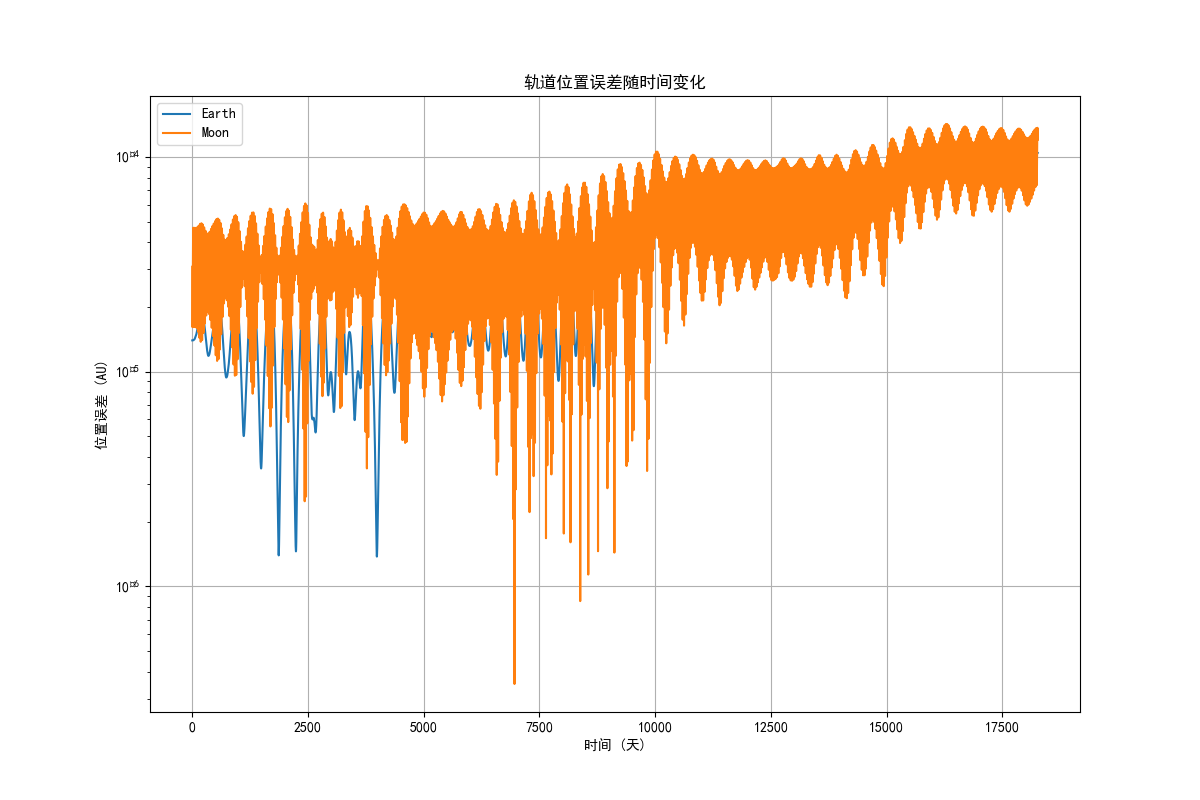
\includegraphics[width=0.5\linewidth]{images/position_errors.png}
    \caption{对照组(预测准确率96.70\%)}
    \label{fig:position_error}
\end{figure}

在此基础上,我们对参数的影响进行了粗略的估计。在程序中影响模拟结果的参数主要包括时间步长、天体数量和各类天文常数。
由于最终结果对参数的依赖关系非常复杂,我们采用微调参数的值来估计参数的误差对结果有多大影响。\\
在具体陈列实验结果之前,需要说明:由于我们的最终目标是预测日/月食的时间而非模拟太阳系内天体的运动,应该将最后模拟的精度和正确率作为唯一的评价标准,而非单独追求三个天体位置的正确性。
所以,在所有实验中,我们均以最后得到的日/月食时间误差而非天体位置作为评价标准。
首先是时间步长,模拟发现不同时间步长下的误差分布如图\ref{fig:eclipse_error_0.5}、图\ref{fig:eclipse_error_1}、图\ref{fig:eclipse_error_2}所示:

\begin{figure}[H]
    \centering
    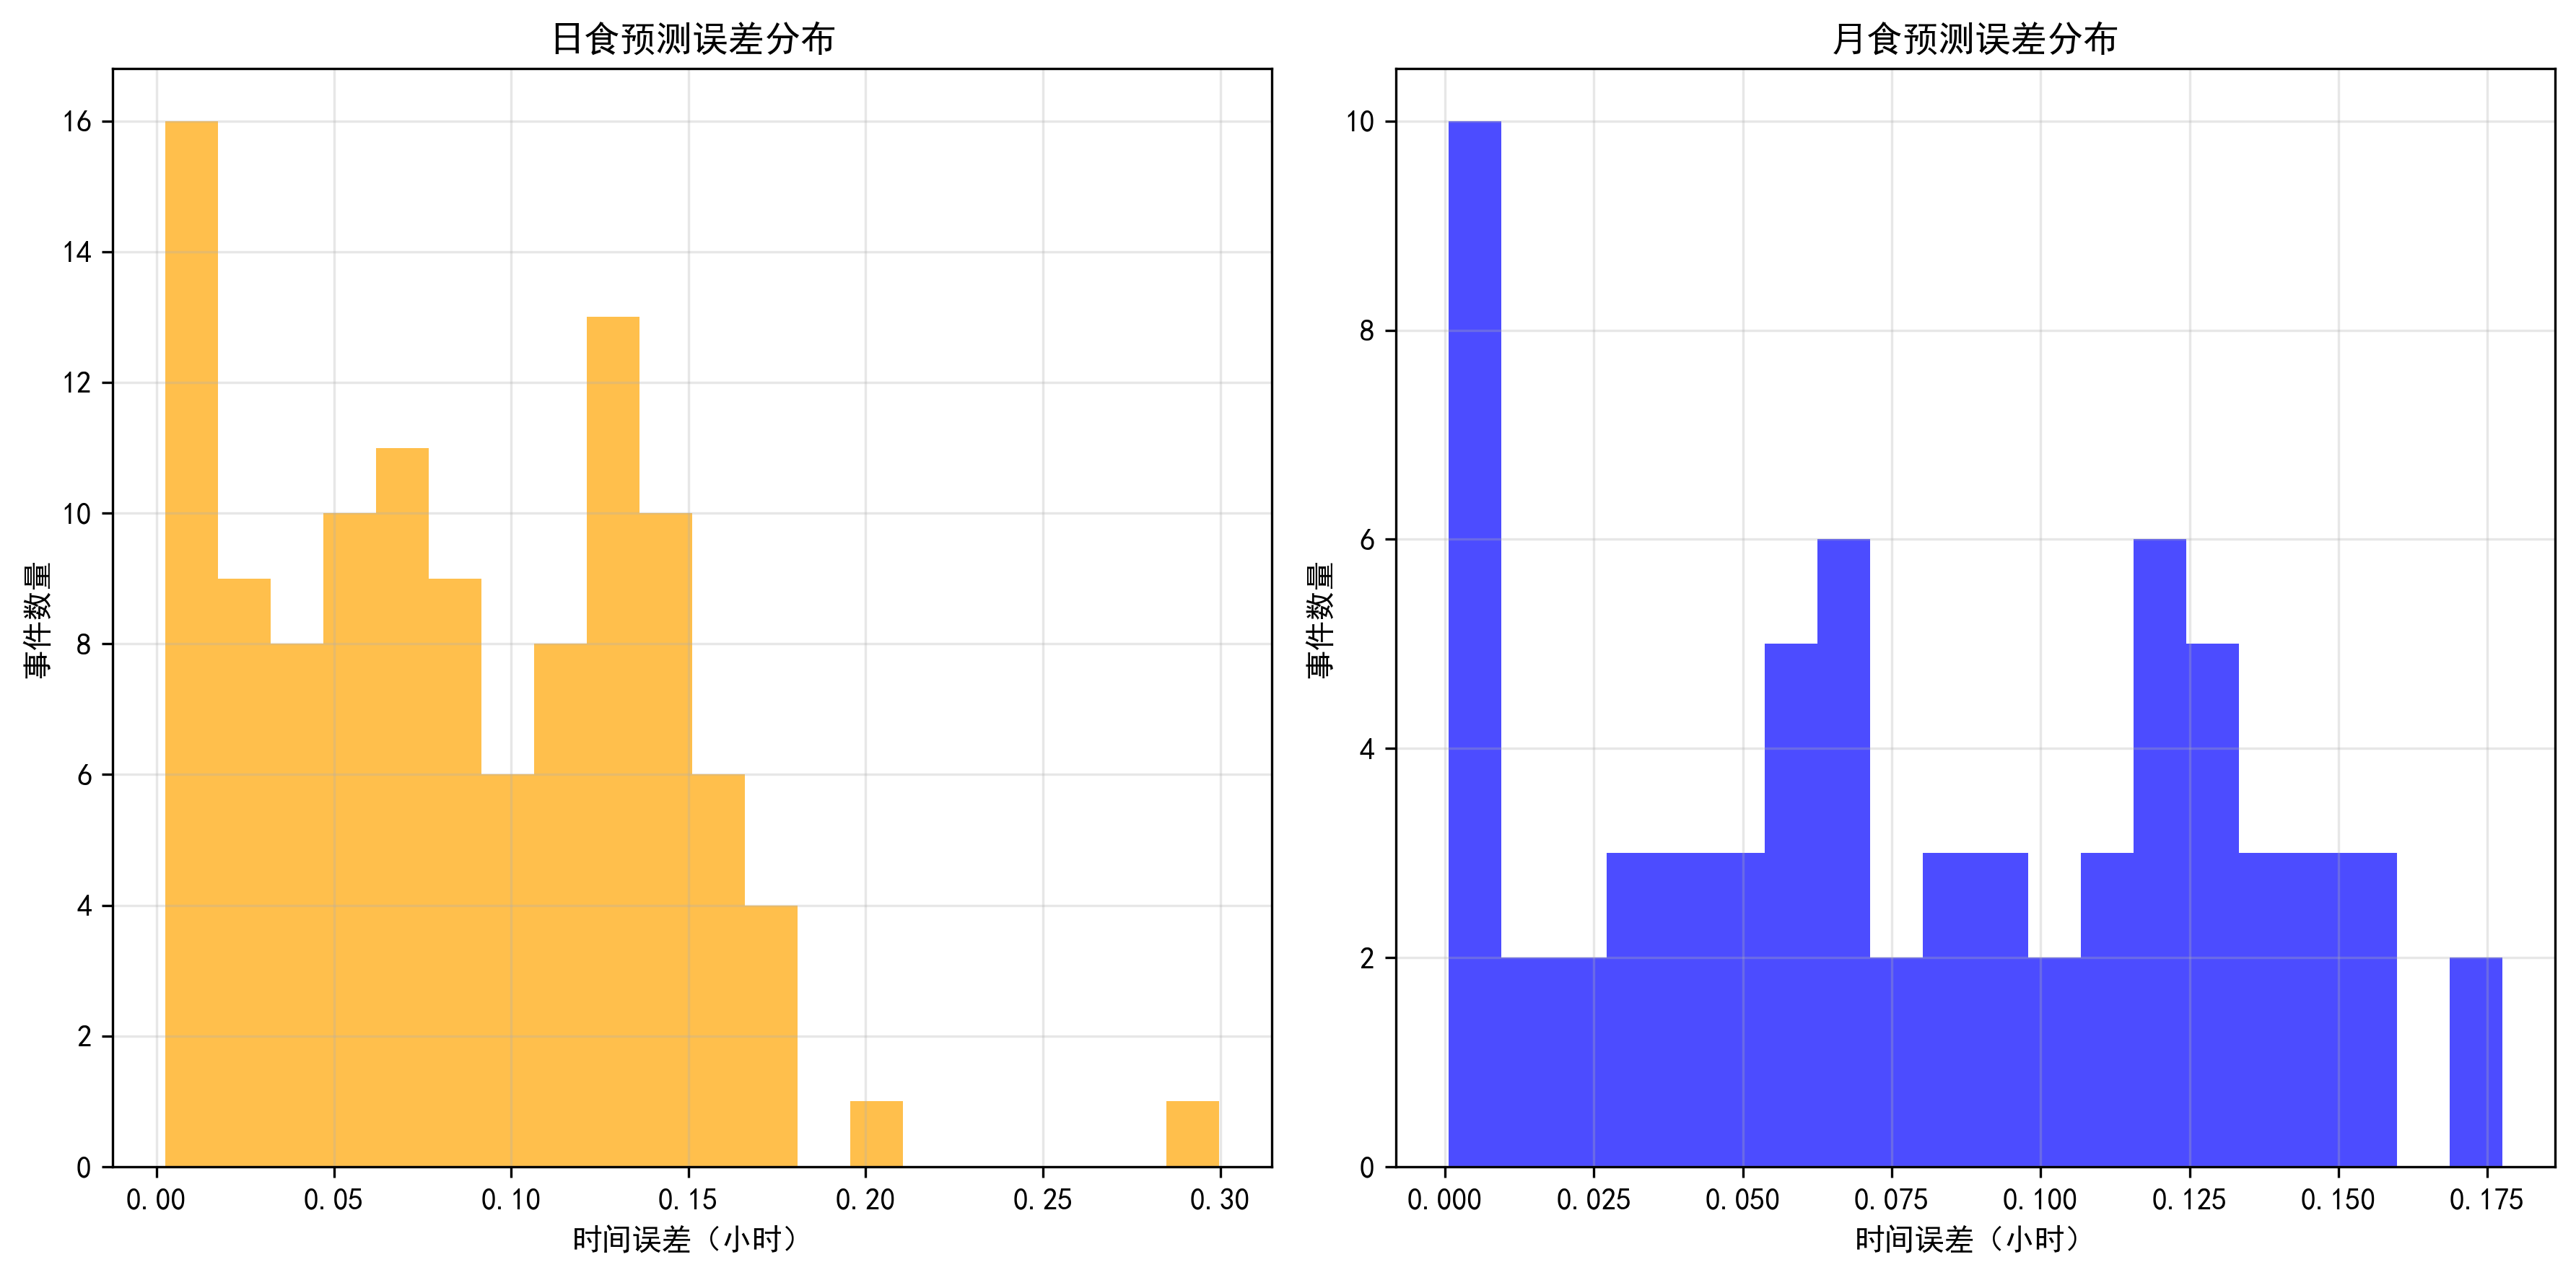
\includegraphics[width=0.5\linewidth]{images/error_distribution_0.5.png}
    \caption{时间步长:0.5(预测准确率:99.45\%)}
    \label{fig:eclipse_error_0.5}
\end{figure}

\begin{figure}[H]
    \centering
    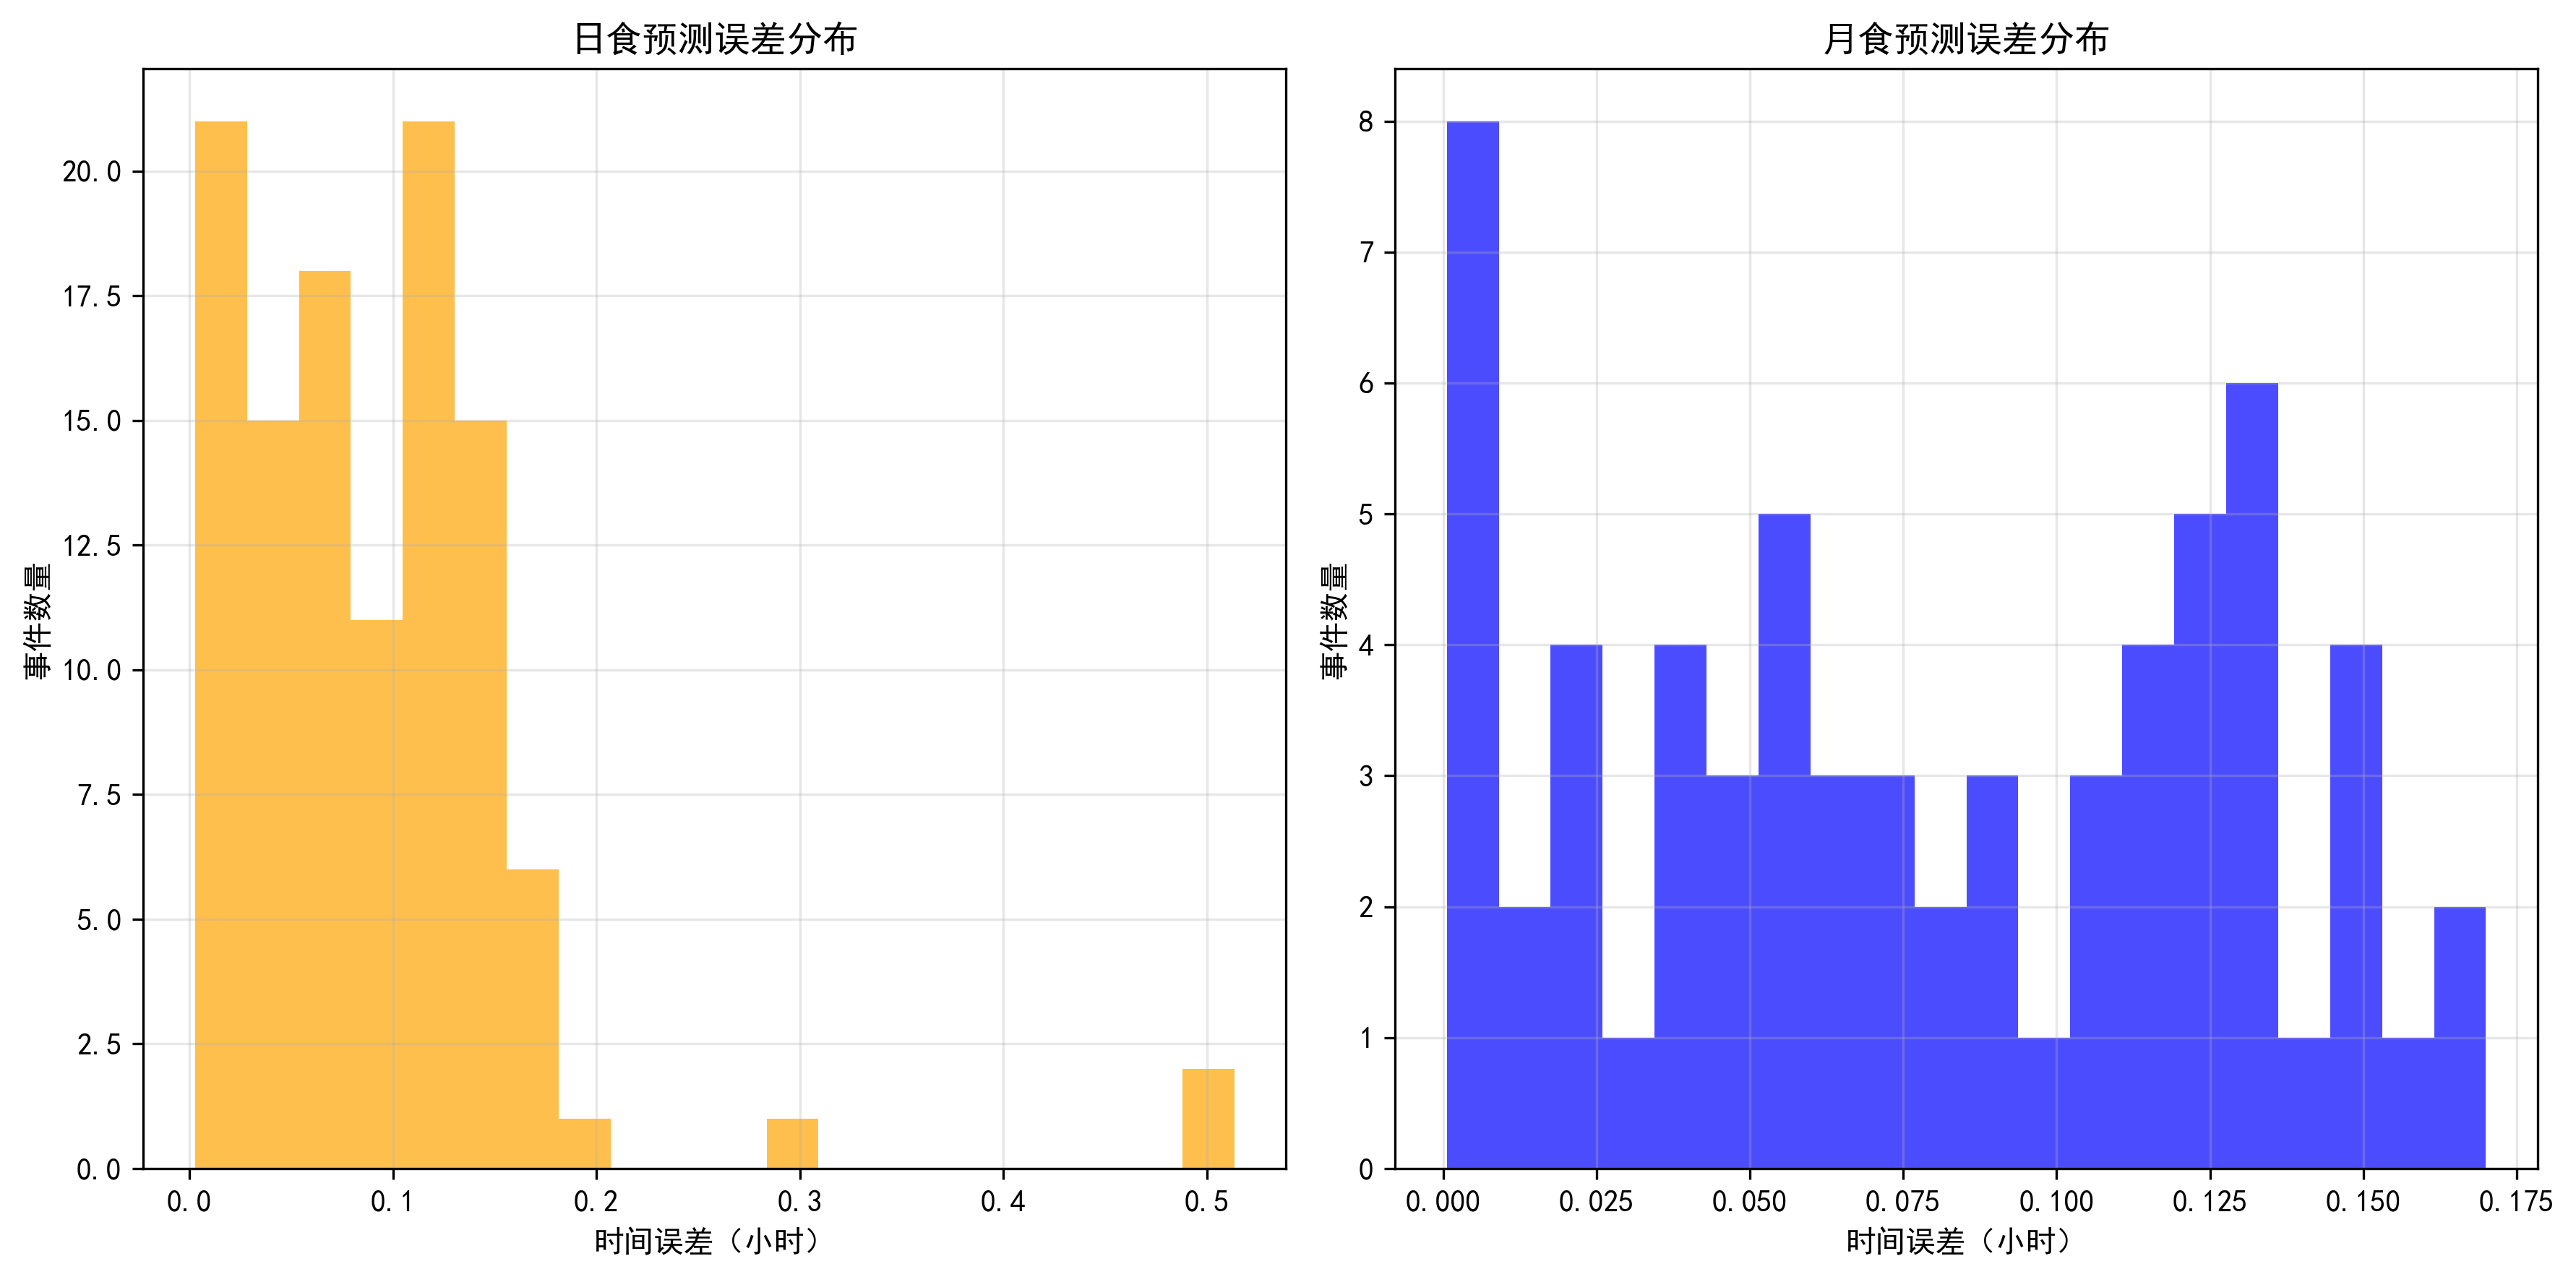
\includegraphics[width=0.5\linewidth]{images/error_distribution_1.png}
    \caption{时间步长:1(预测准确率:96.70\%)}
    \label{fig:eclipse_error_1}
\end{figure}

\begin{figure}[H]
    \centering
    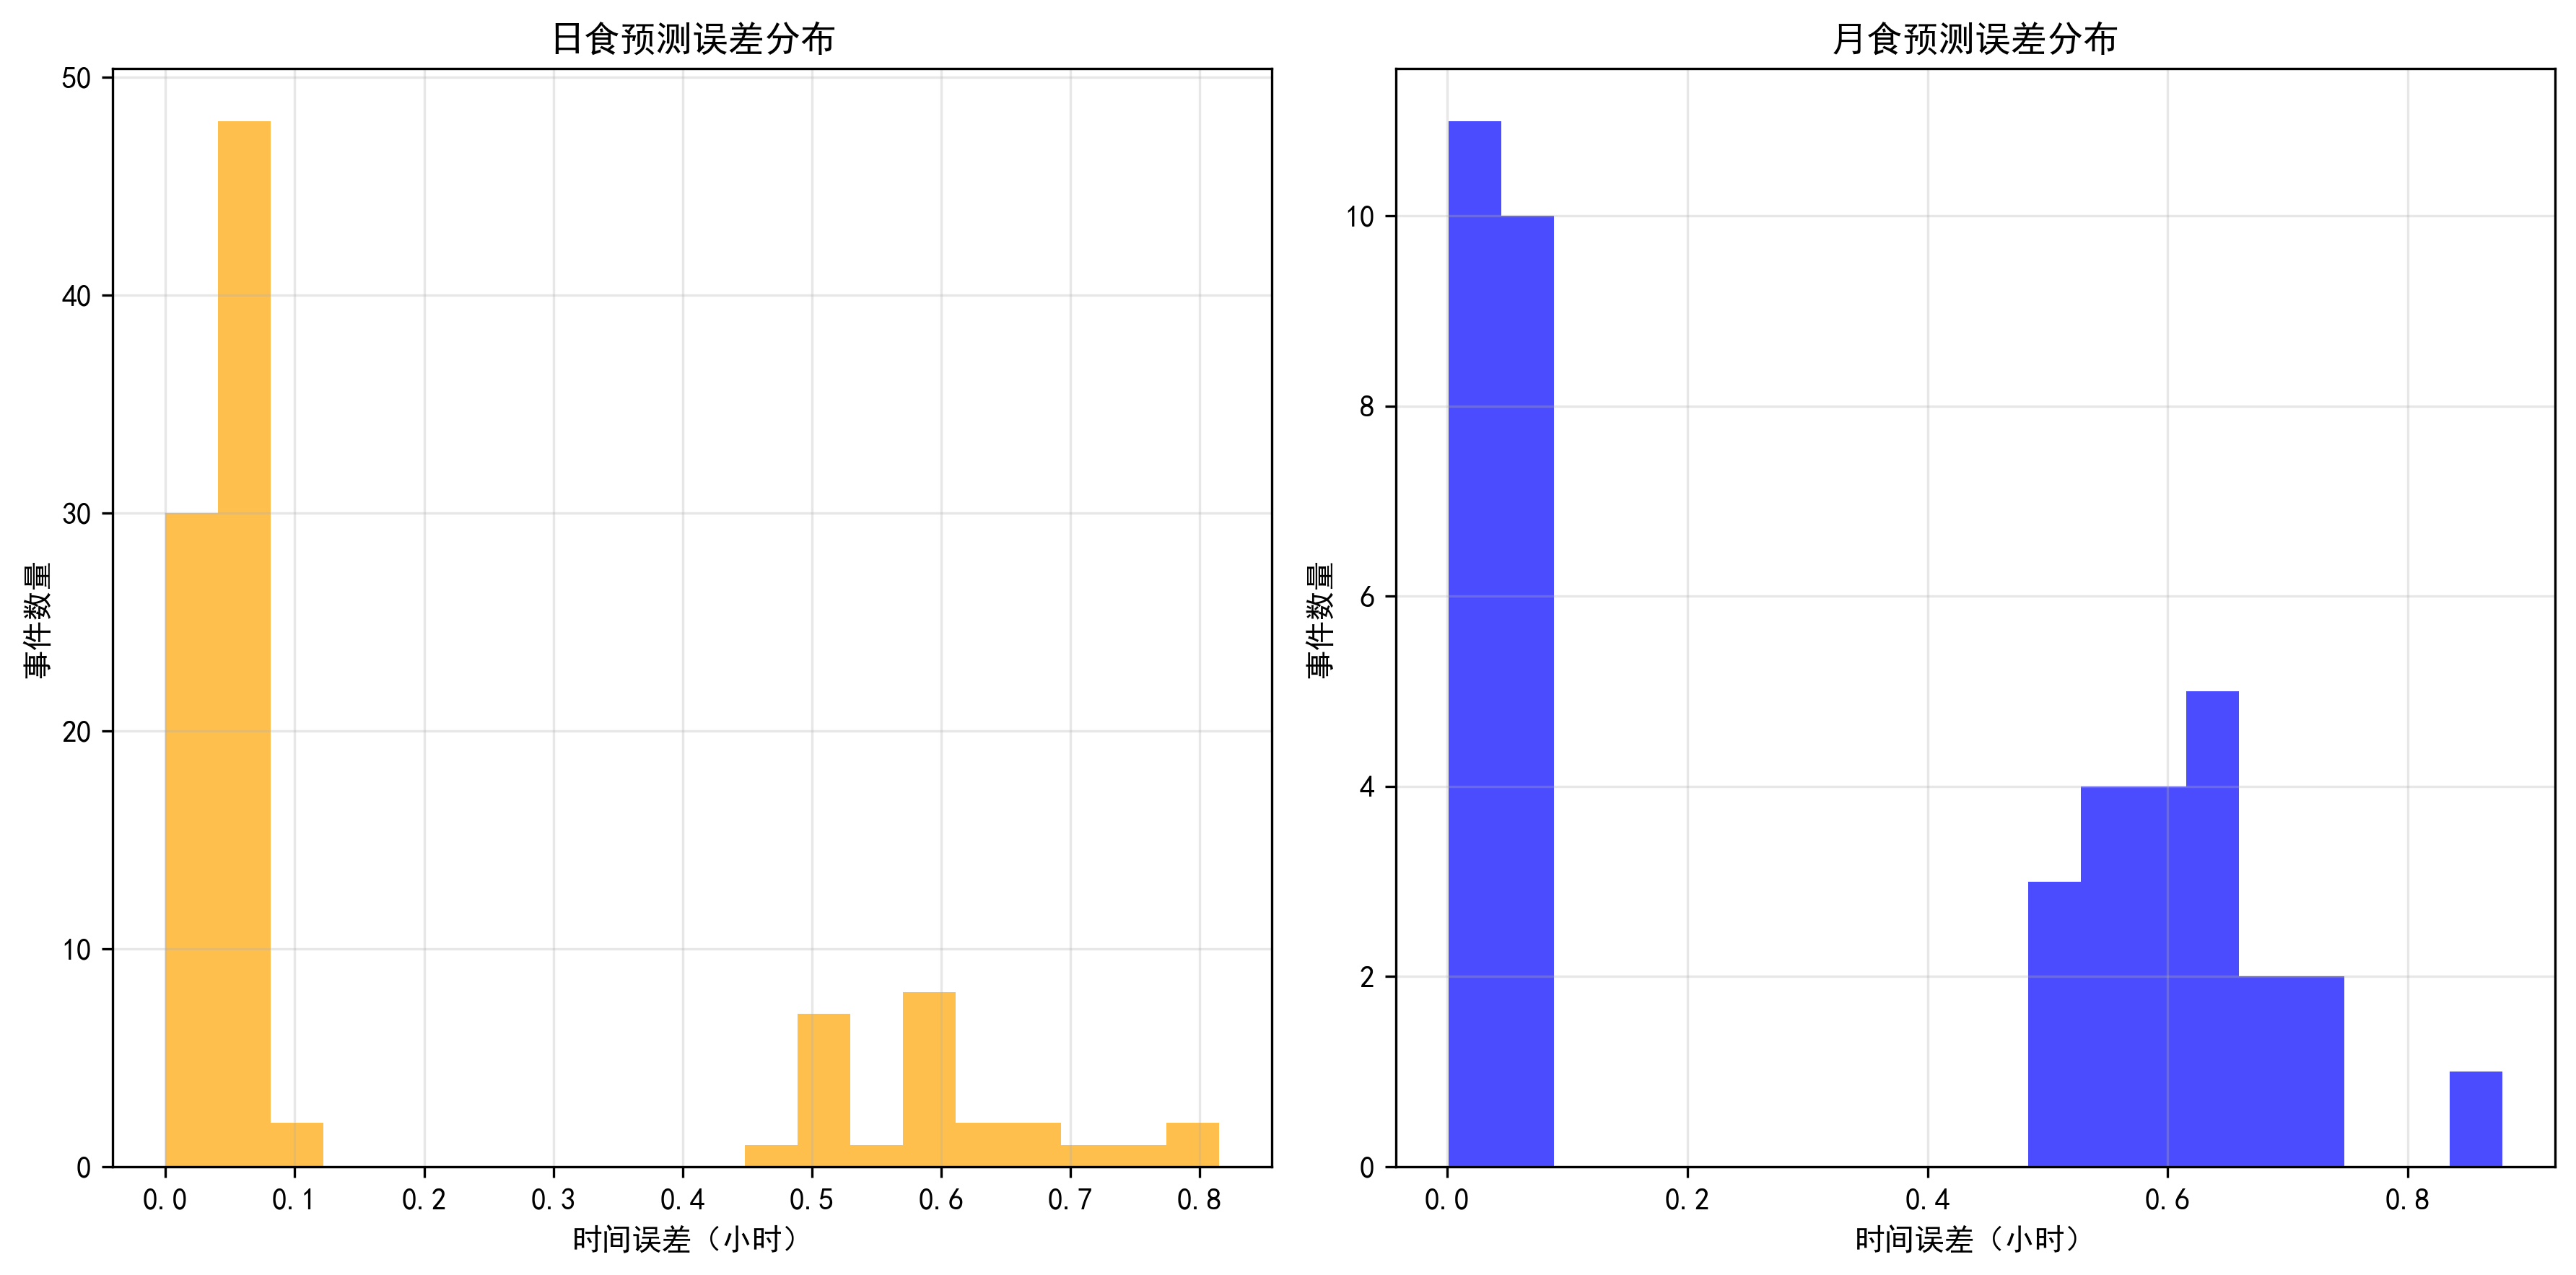
\includegraphics[width=0.5\linewidth]{images/error_distribution_2.png}
    \caption{时间步长:1(预测准确率:80.77\%)}
    \label{fig:eclipse_error_2}
\end{figure}
由此可见,在我们目前的精度下,选取时间步长t=1不会对时间精度产生明显影响,只会略微影响到日/月食判断的准确率(这是因为过长的步长有可能直接跳过一些事件)。
而步长取为2之后则明显看出模拟的精度(无论预测的时间还是准确率)受到了影响。
为方便起见,在以后实验中,若无特殊说明,所有模拟的时间步长均取为1。\\

然后考虑天体数量对模拟的影响,分别在:日地月、日地月+木、日地月+金木、日地月+金木(作为外场)、日地月+金木土,共五种设定下进行实验。
得到结果如图\ref{fig:eclipse_error_sem}、图\ref{fig:eclipse_error_semj}、图\ref{fig:eclipse_error_semjv}、图\ref{fig:eclipse_error_semjv_aux}、图\ref{fig:eclipse_error_semjvs_aux}所示:
\begin{figure}[h]
    \centering
    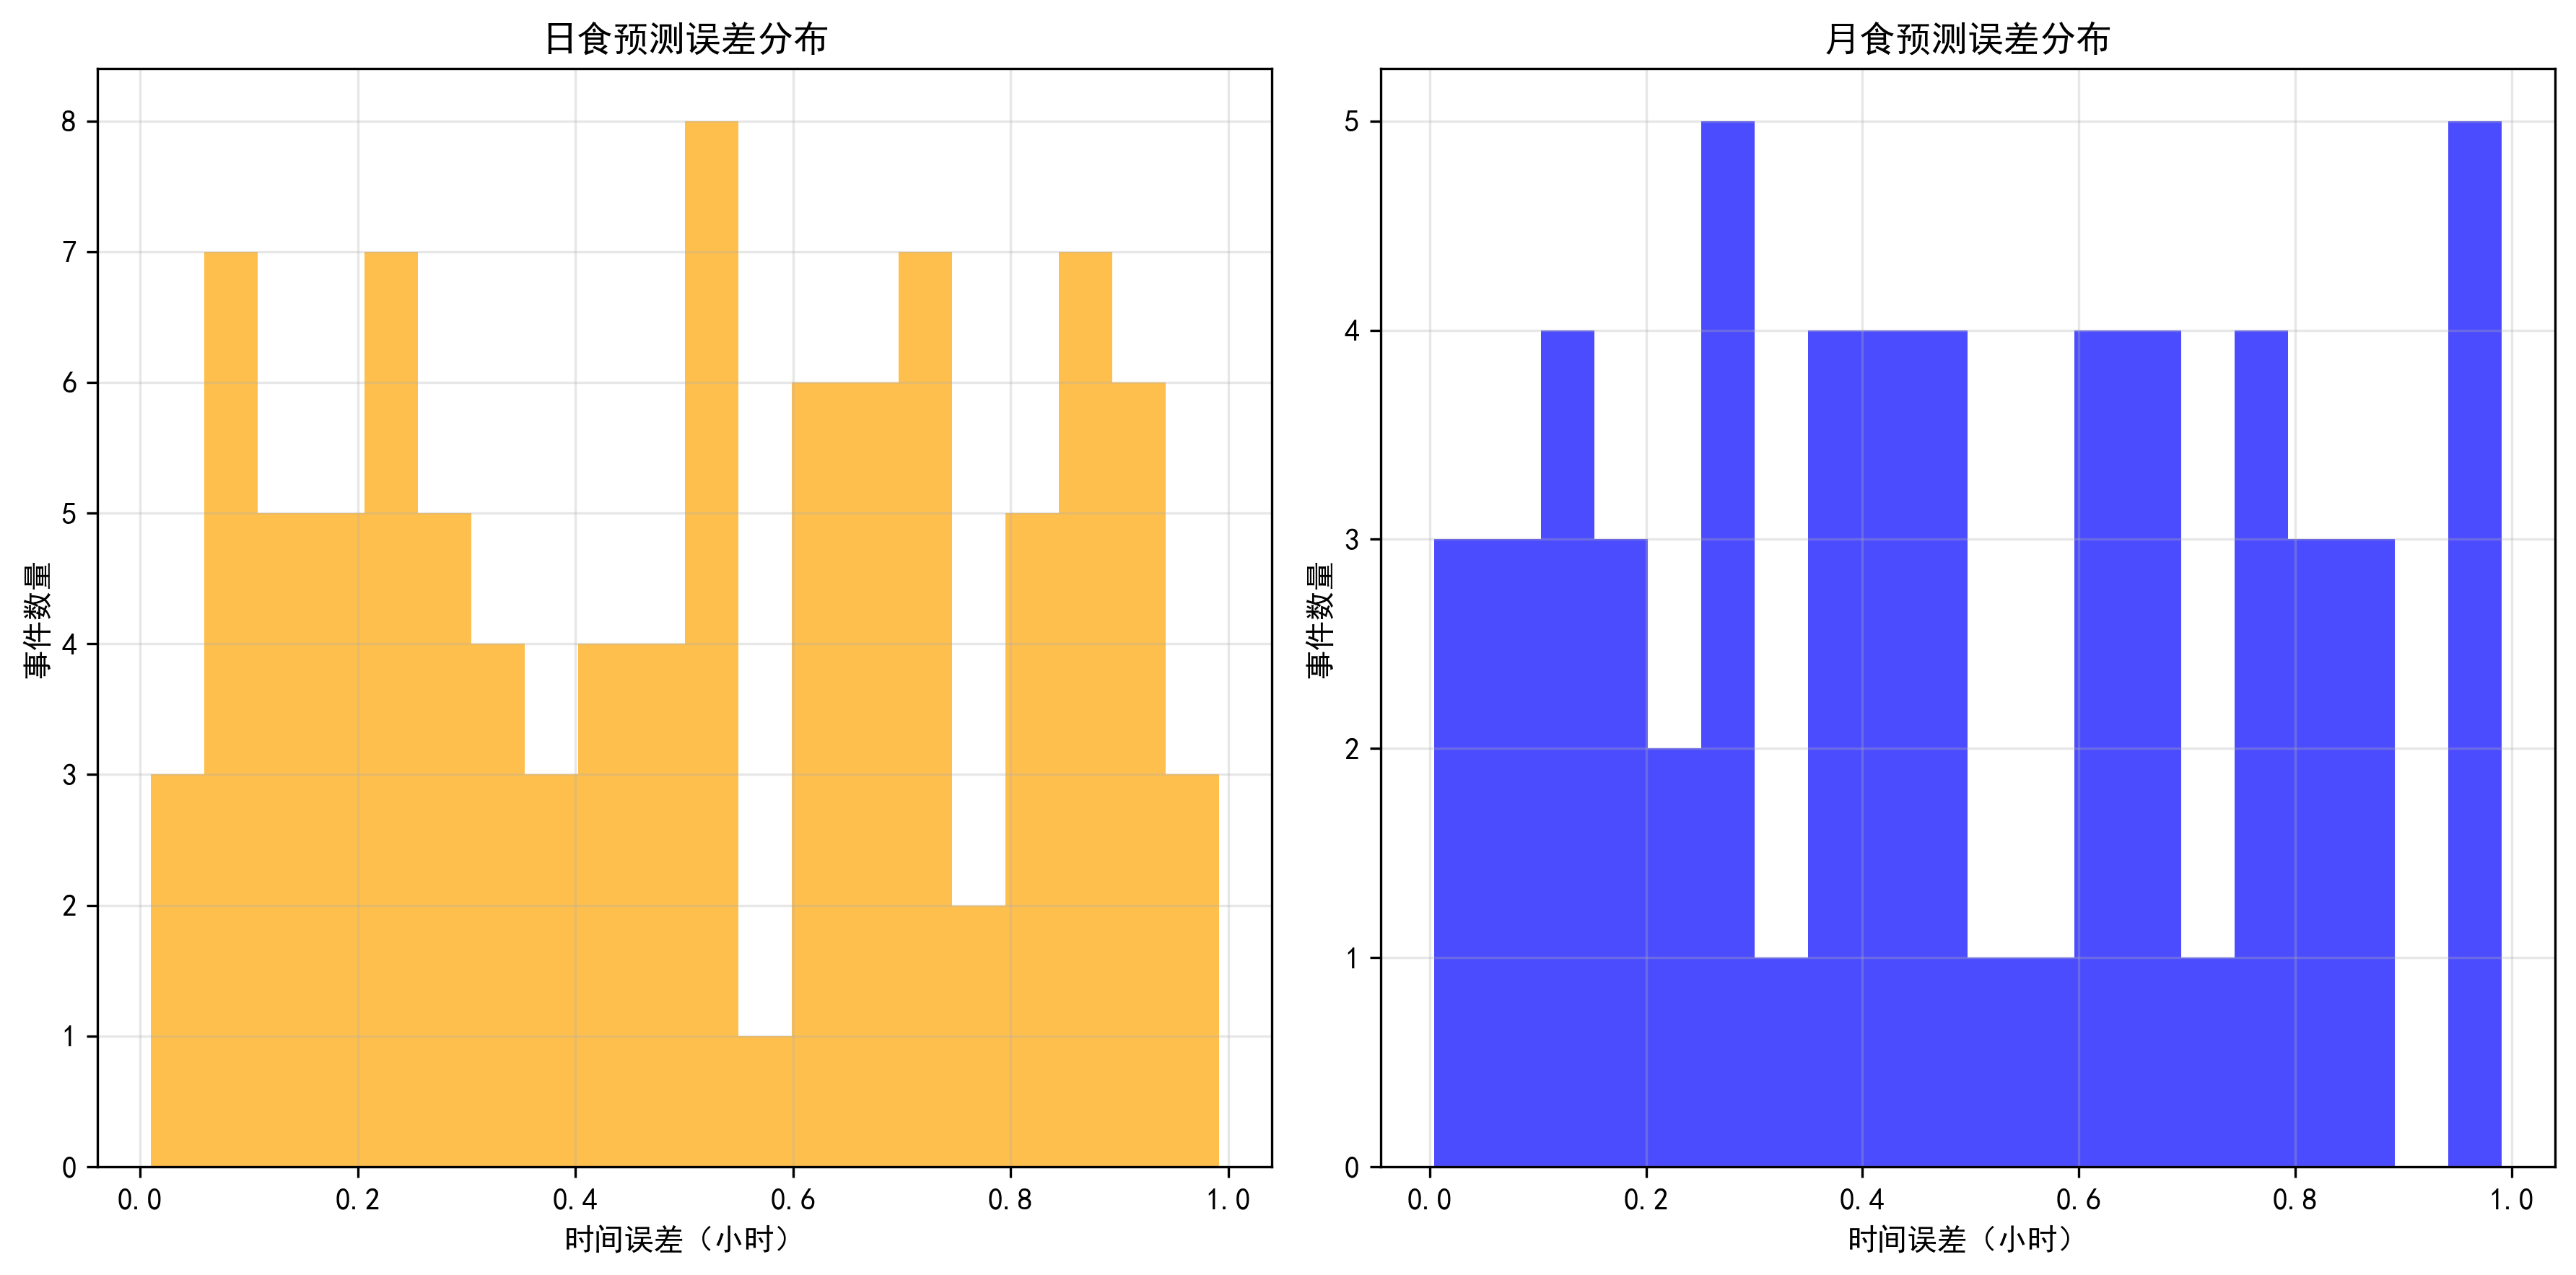
\includegraphics[width=0.5\linewidth]{images/error_distribution_sem.png}
    \caption{体系:日地月(预测准确率:86.26\%)}
    \label{fig:eclipse_error_sem}
\end{figure}

\begin{figure}[H]
    \centering
    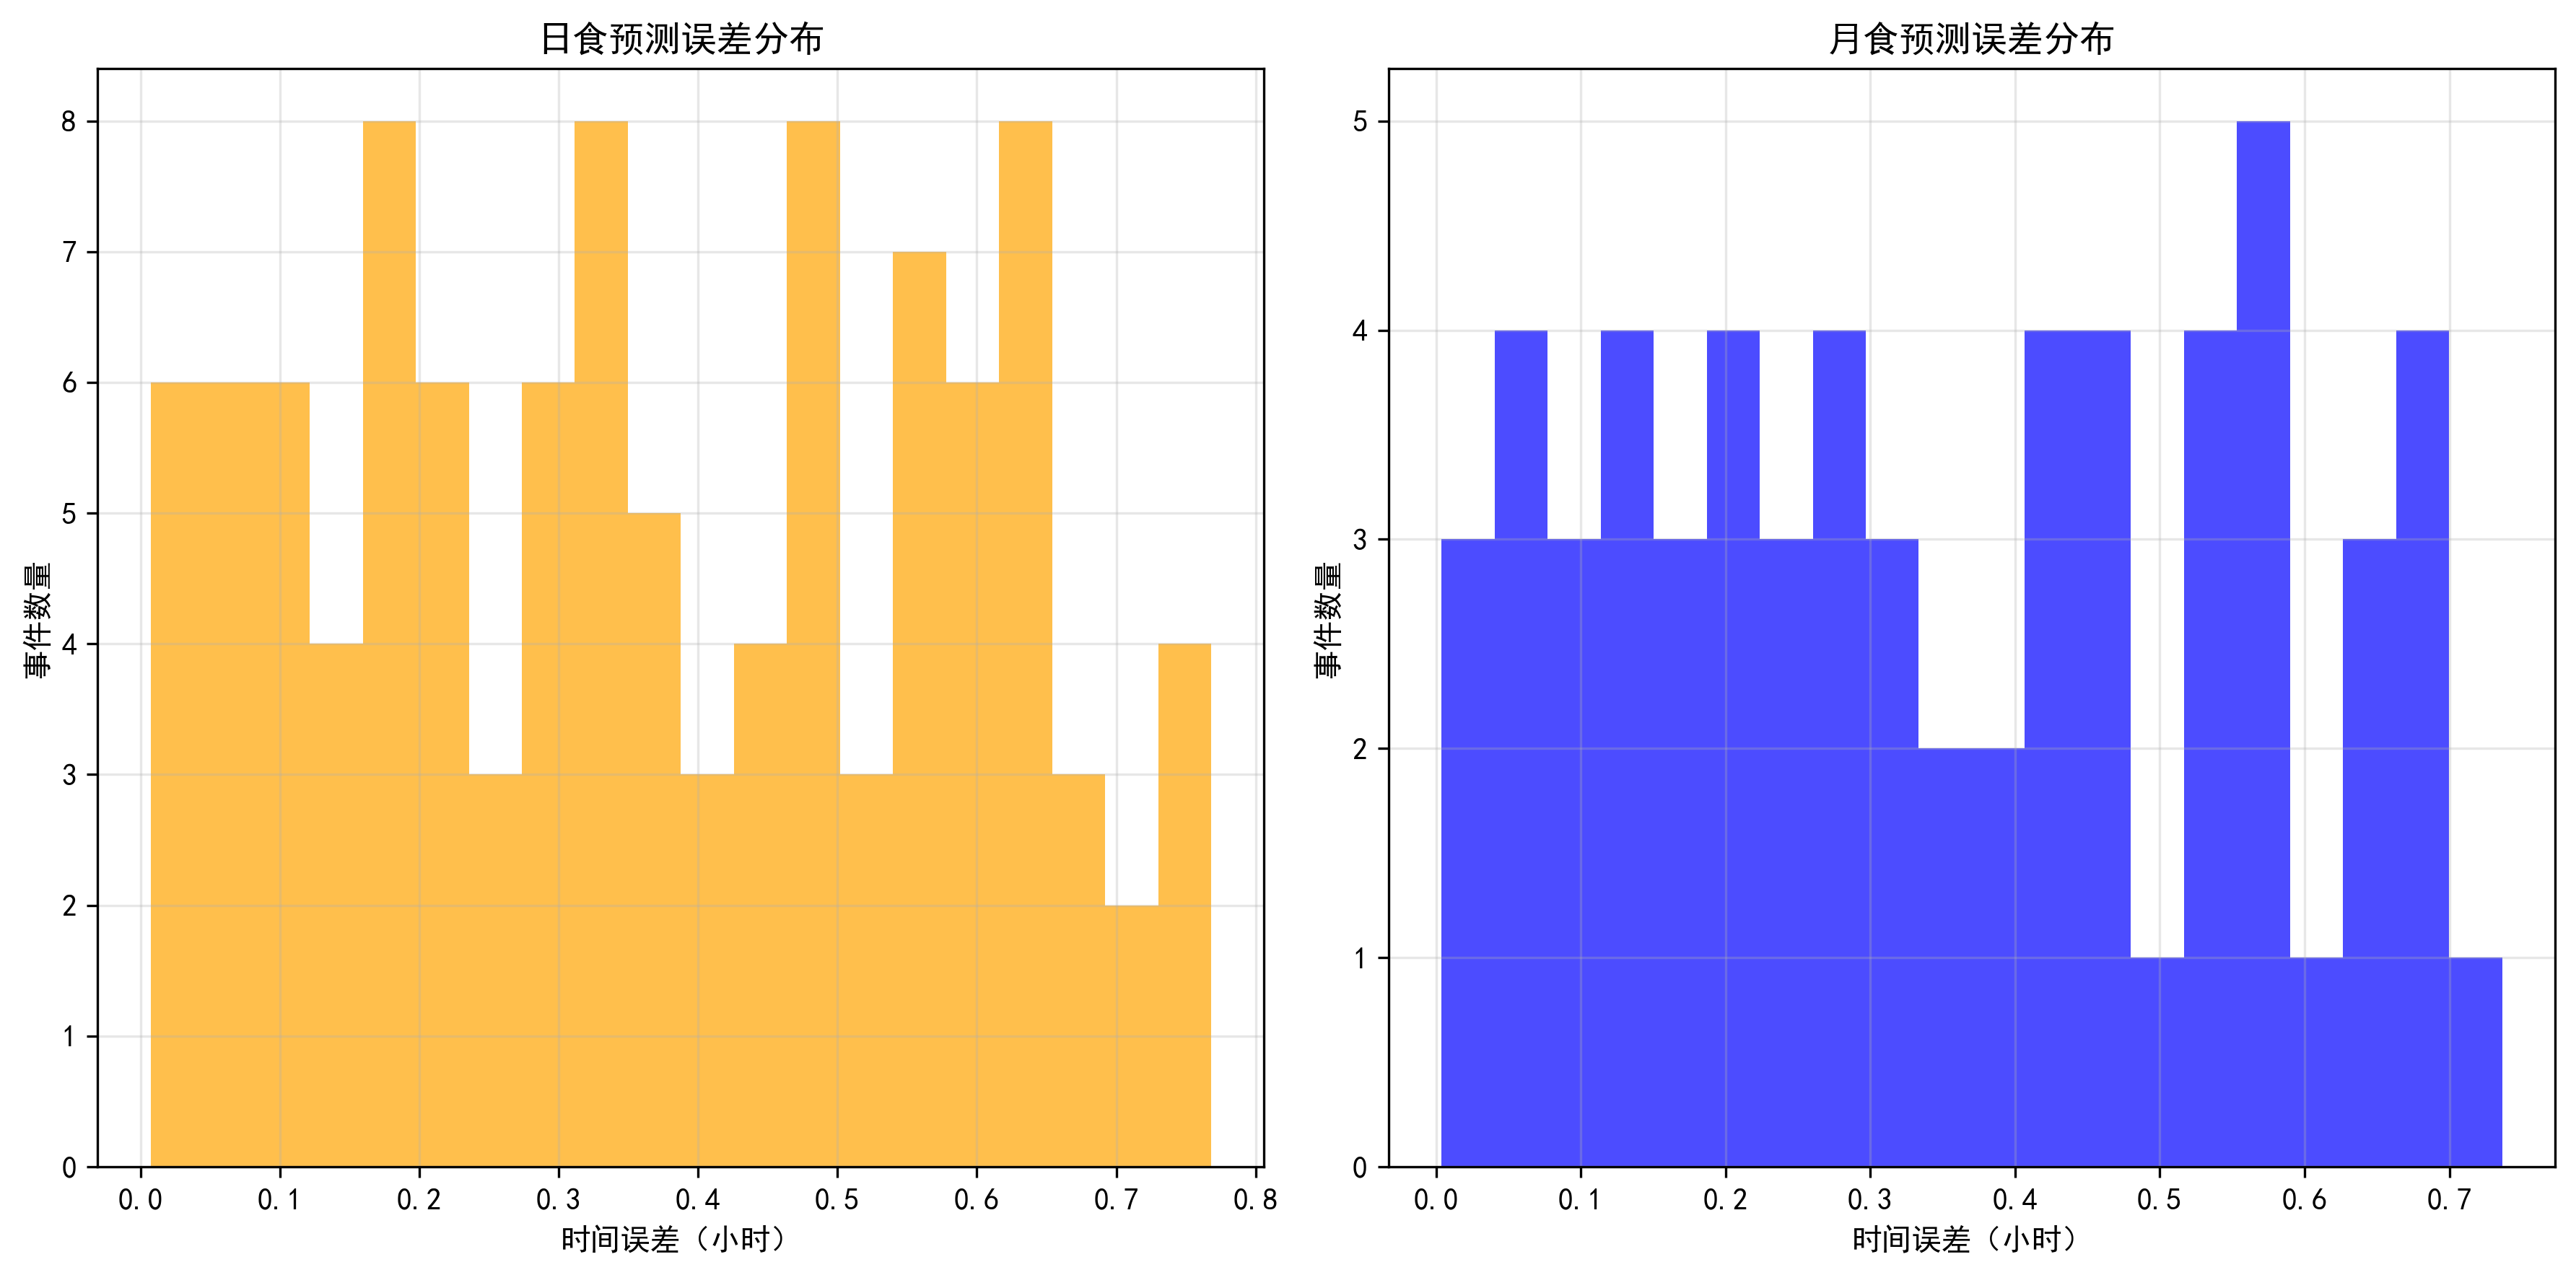
\includegraphics[width=0.5\linewidth]{images/error_distribution_semj.png}
    \caption{体系:日地月+木(预测准确率:92.31\%)}
    \label{fig:eclipse_error_semj}
\end{figure}

\begin{figure}[H]
    \centering
    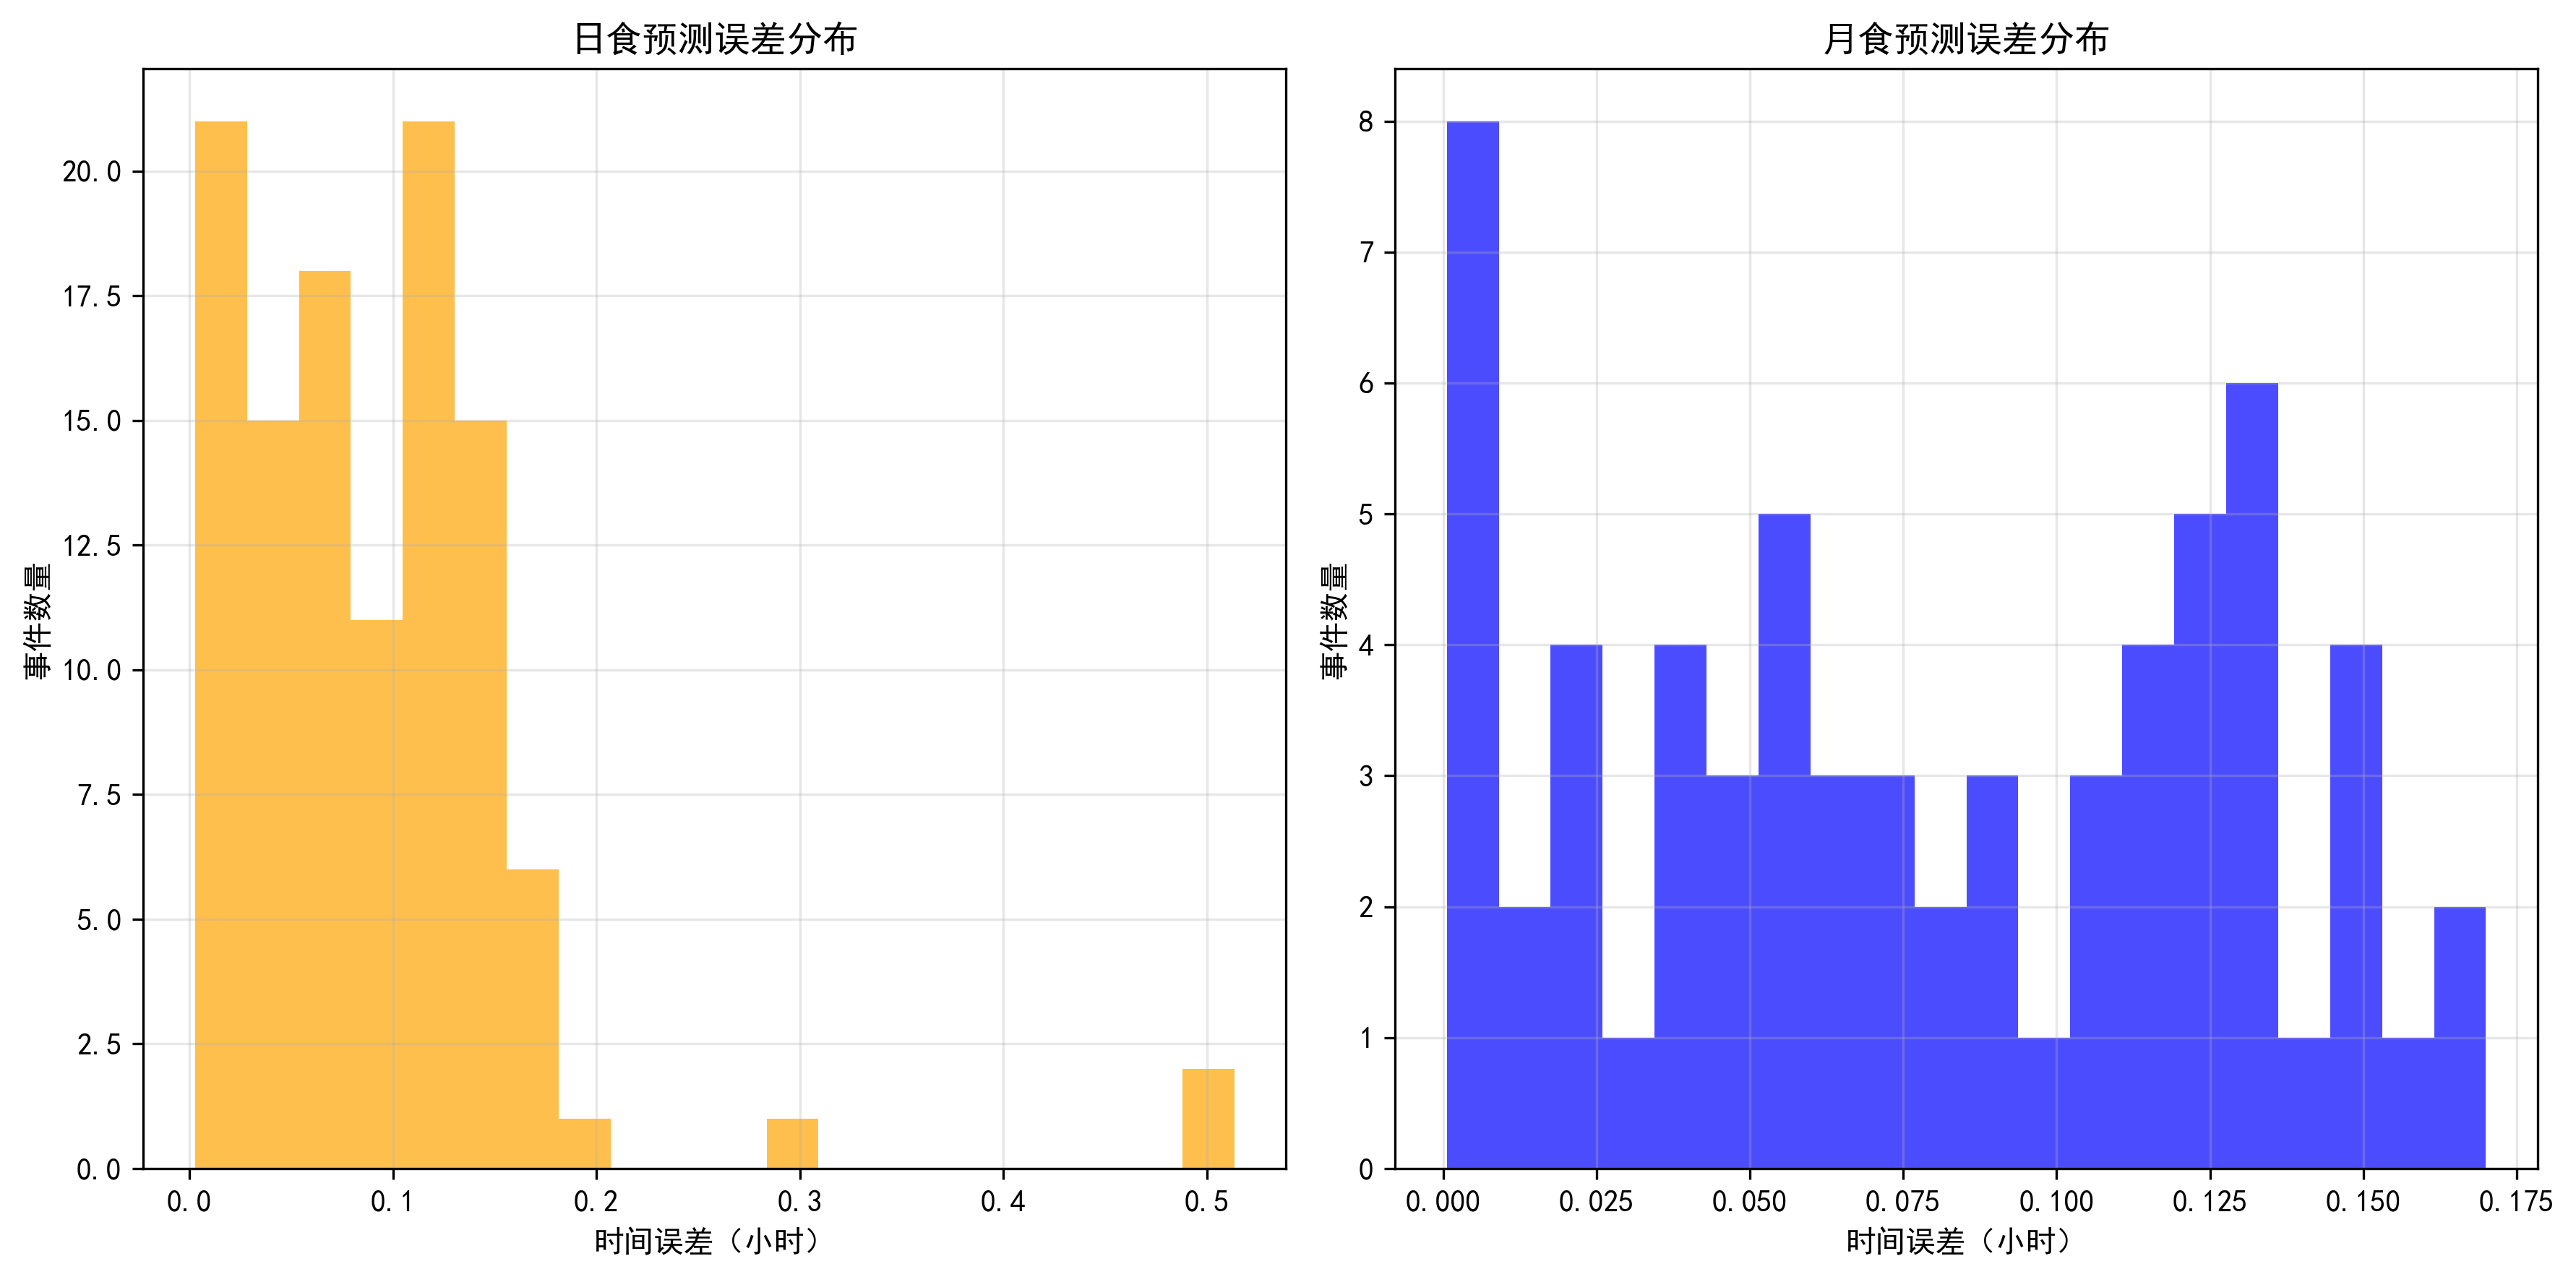
\includegraphics[width=0.5\linewidth]{images/error_distribution_1.png}
    \caption{体系:日地月+金木(预测准确率:96.70\%)}
    \label{fig:eclipse_error_semjv}
\end{figure}

\begin{figure}[H]
    \centering
    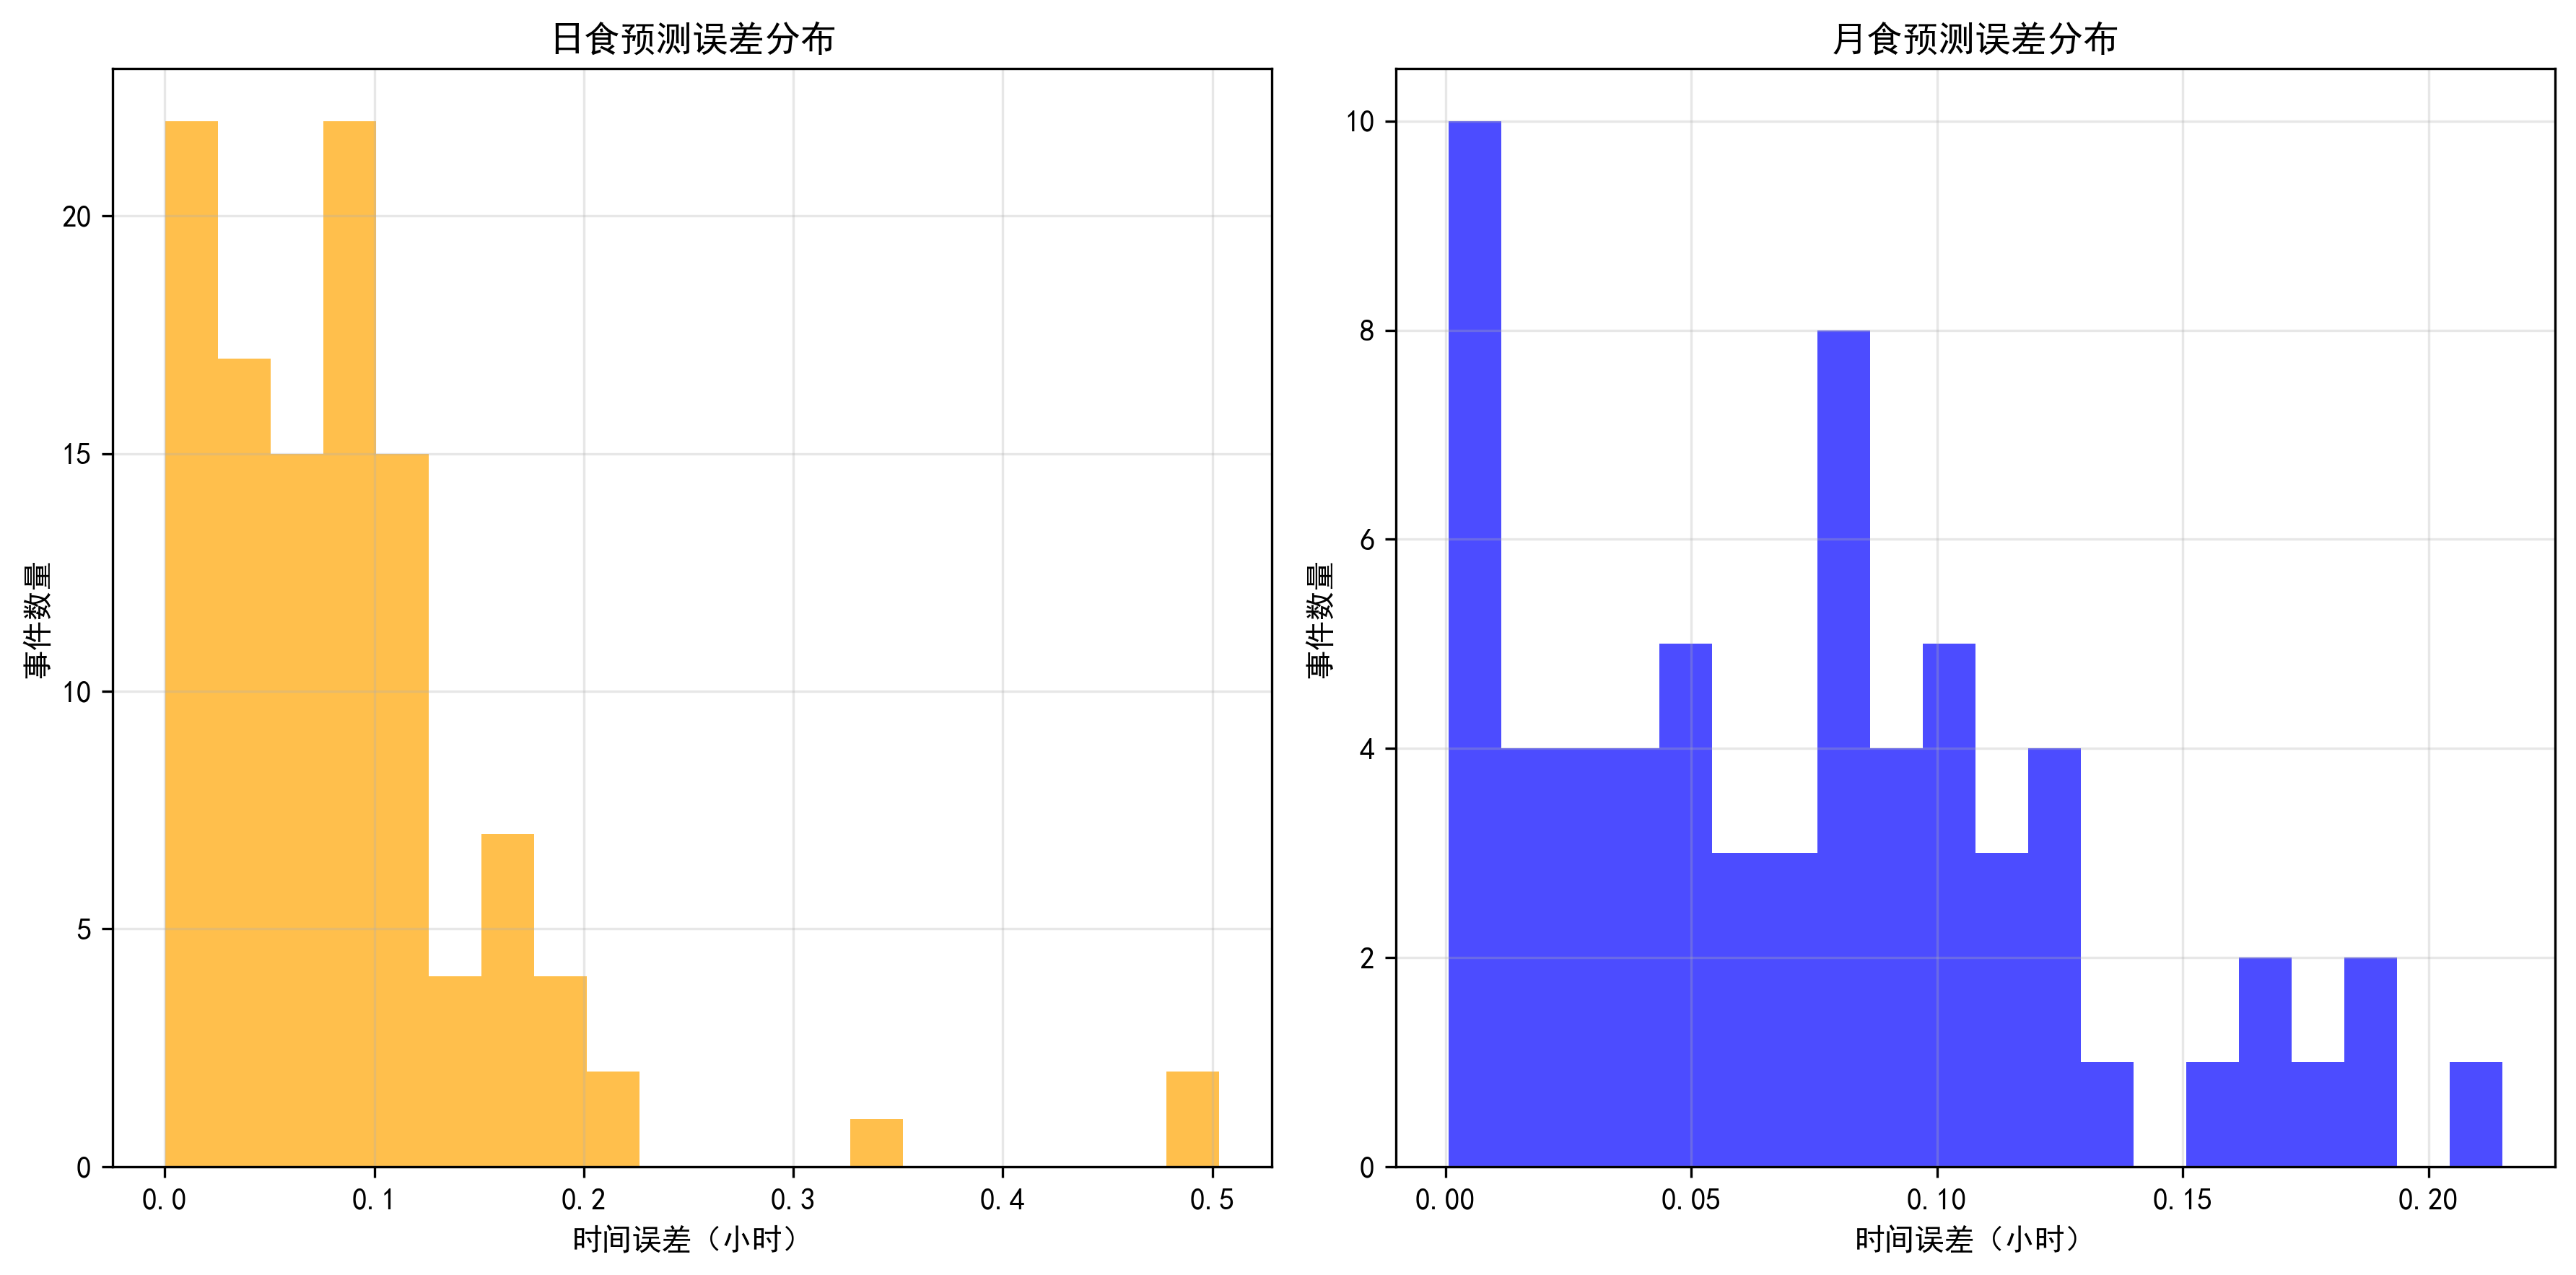
\includegraphics[width=0.5\linewidth]{images/error_distribution_semjv_aux.png}
    \caption{体系:日地月+金木(作为外场)(预测准确率:96.70\%)}
    \label{fig:eclipse_error_semjv_aux}
\end{figure}

\begin{figure}[H]
    \centering
    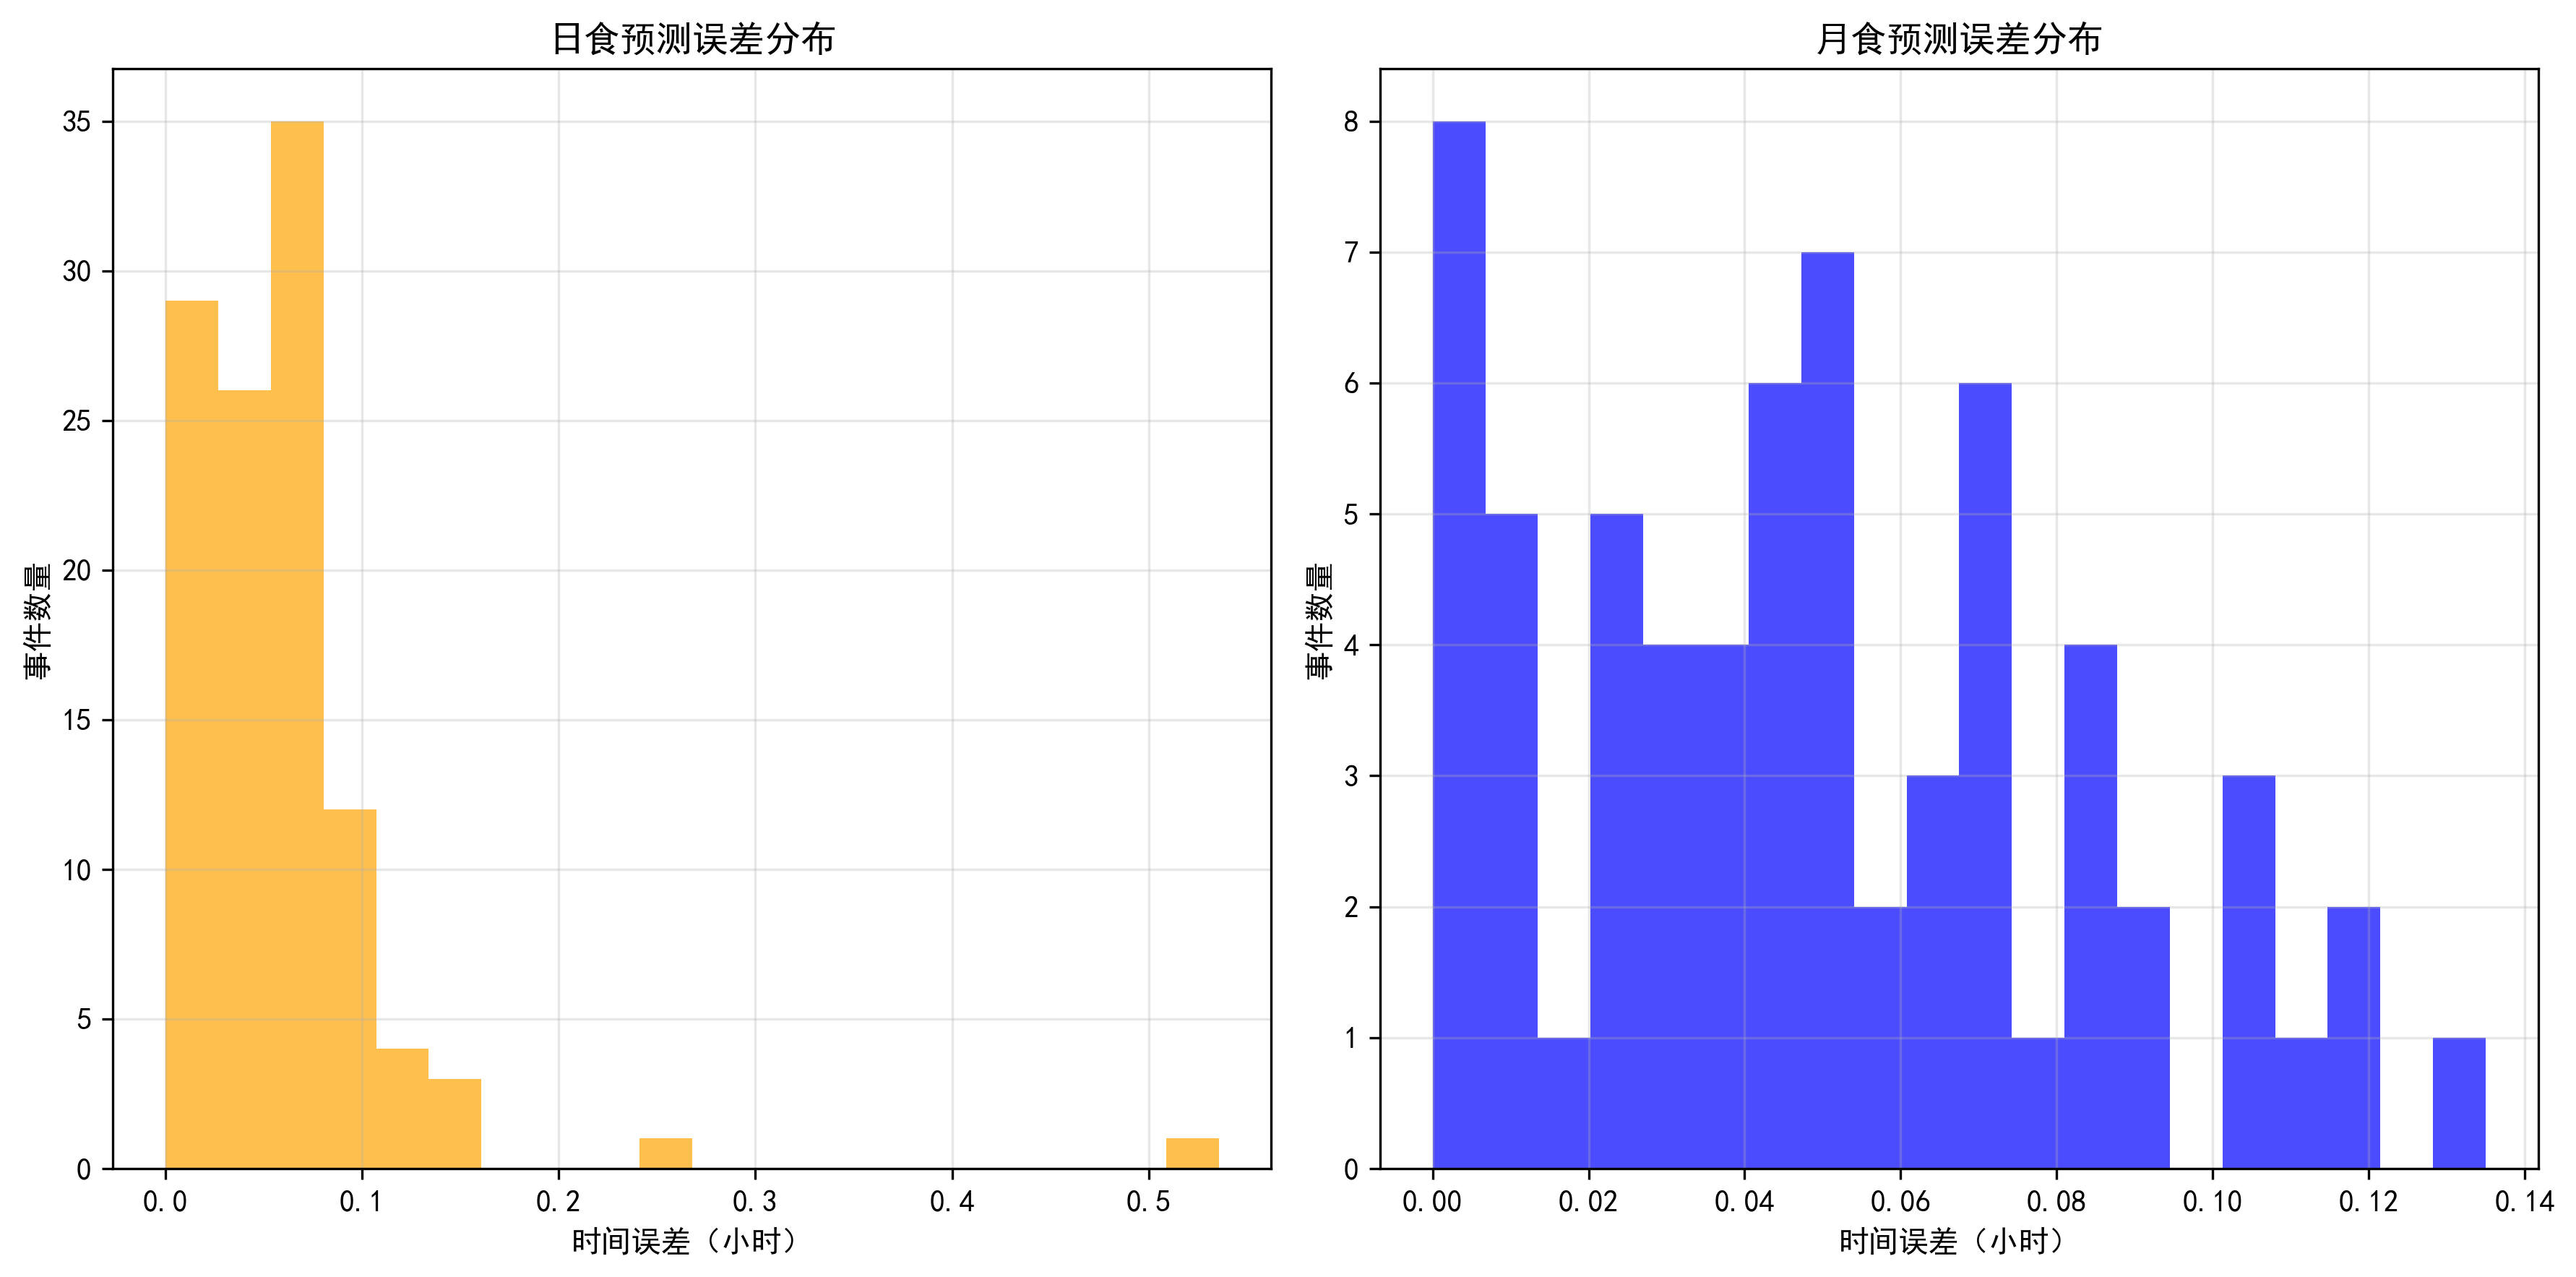
\includegraphics[width=0.5\linewidth]{images/error_distribution_semjvs_aux.png}
    \caption{体系:日地月+金木土(作为外场)(预测准确率:96.70\%)}
    \label{fig:eclipse_error_semjvs_aux}
\end{figure}

由此可见,木星和金星均对预测结果有着明显的影响,在此基础上,将大行星的影响作为外场考虑并不会带来明显的误差,并且这个近似带来的准确率损失远不如能够进一步添加其他行星系统带来的收益。\\
最后考虑天文常数对结果的影响,对天体的质量作量级为$10^{-7}$量级的扰动,观察结果,如图\ref{fig:eclipse_error_sun}、图\ref{fig:eclipse_error_earth}、图\ref{fig:eclipse_error_moon}:
\begin{figure}[h]
    \centering
    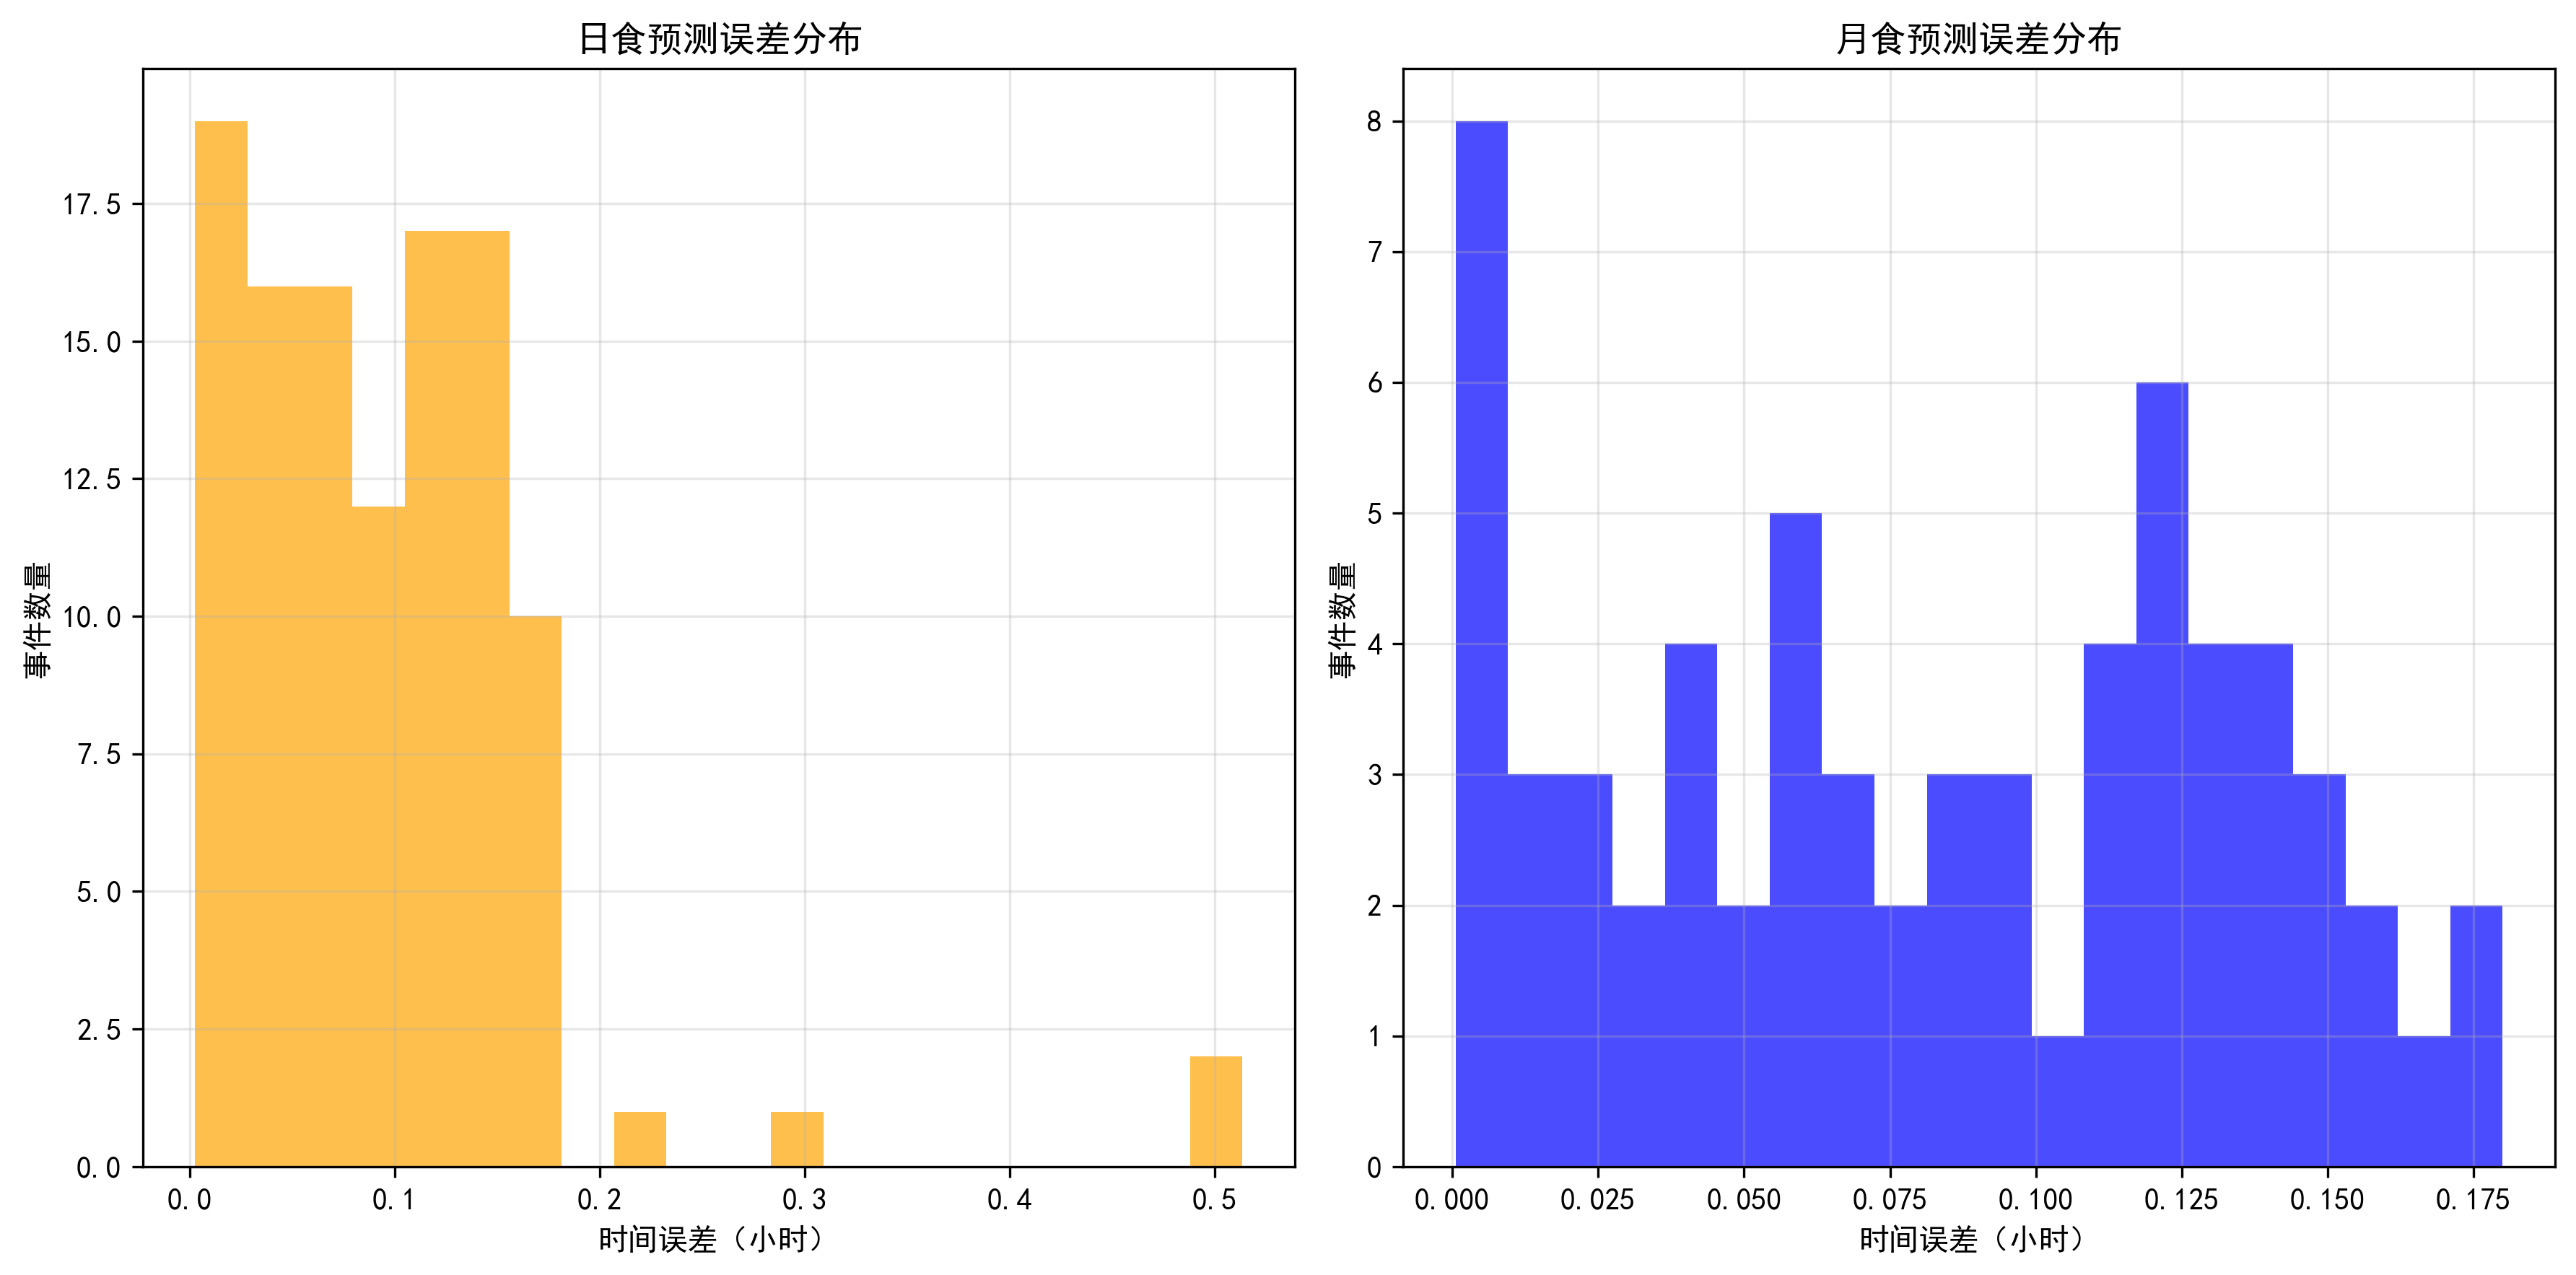
\includegraphics[width=0.5\linewidth]{images/error_distribution_sun.png}
    \caption{扰动对象:太阳质量(预测准确率:96.70\%)}
    \label{fig:eclipse_error_sun}
\end{figure}

\begin{figure}[H]
    \centering
    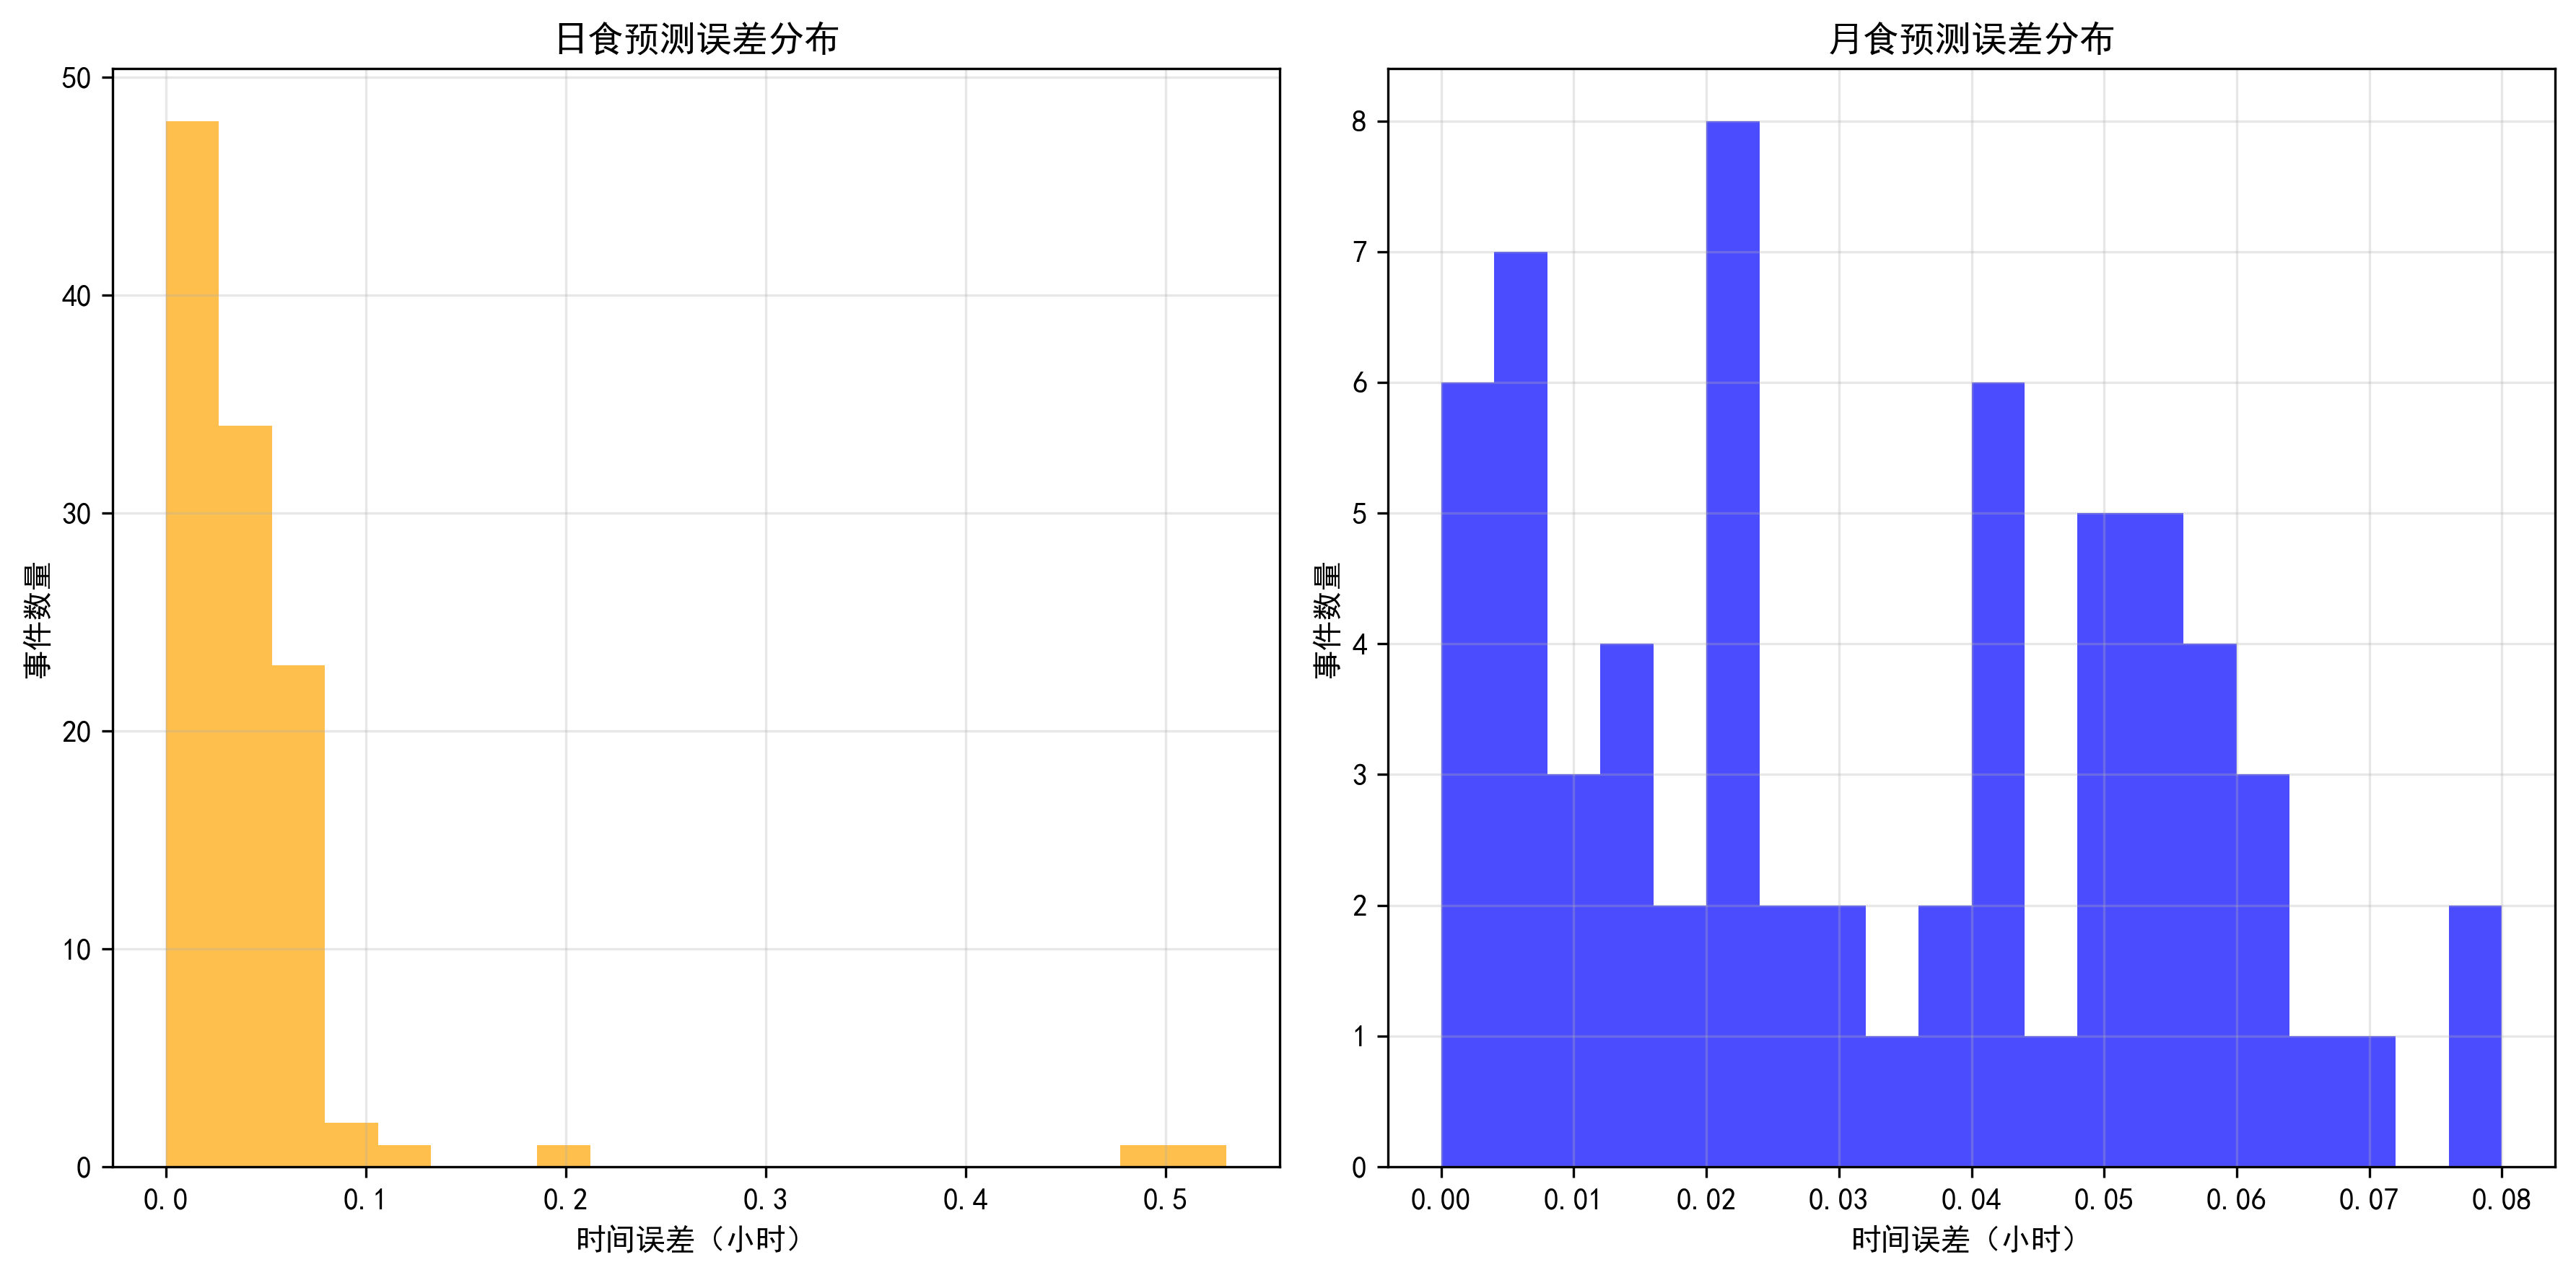
\includegraphics[width=0.5\linewidth]{images/error_distribution_earth.png}
    \caption{扰动对象:地球质量(预测准确率:96.70\%)}
    \label{fig:eclipse_error_earth}
\end{figure}

\begin{figure}[H]
    \centering
    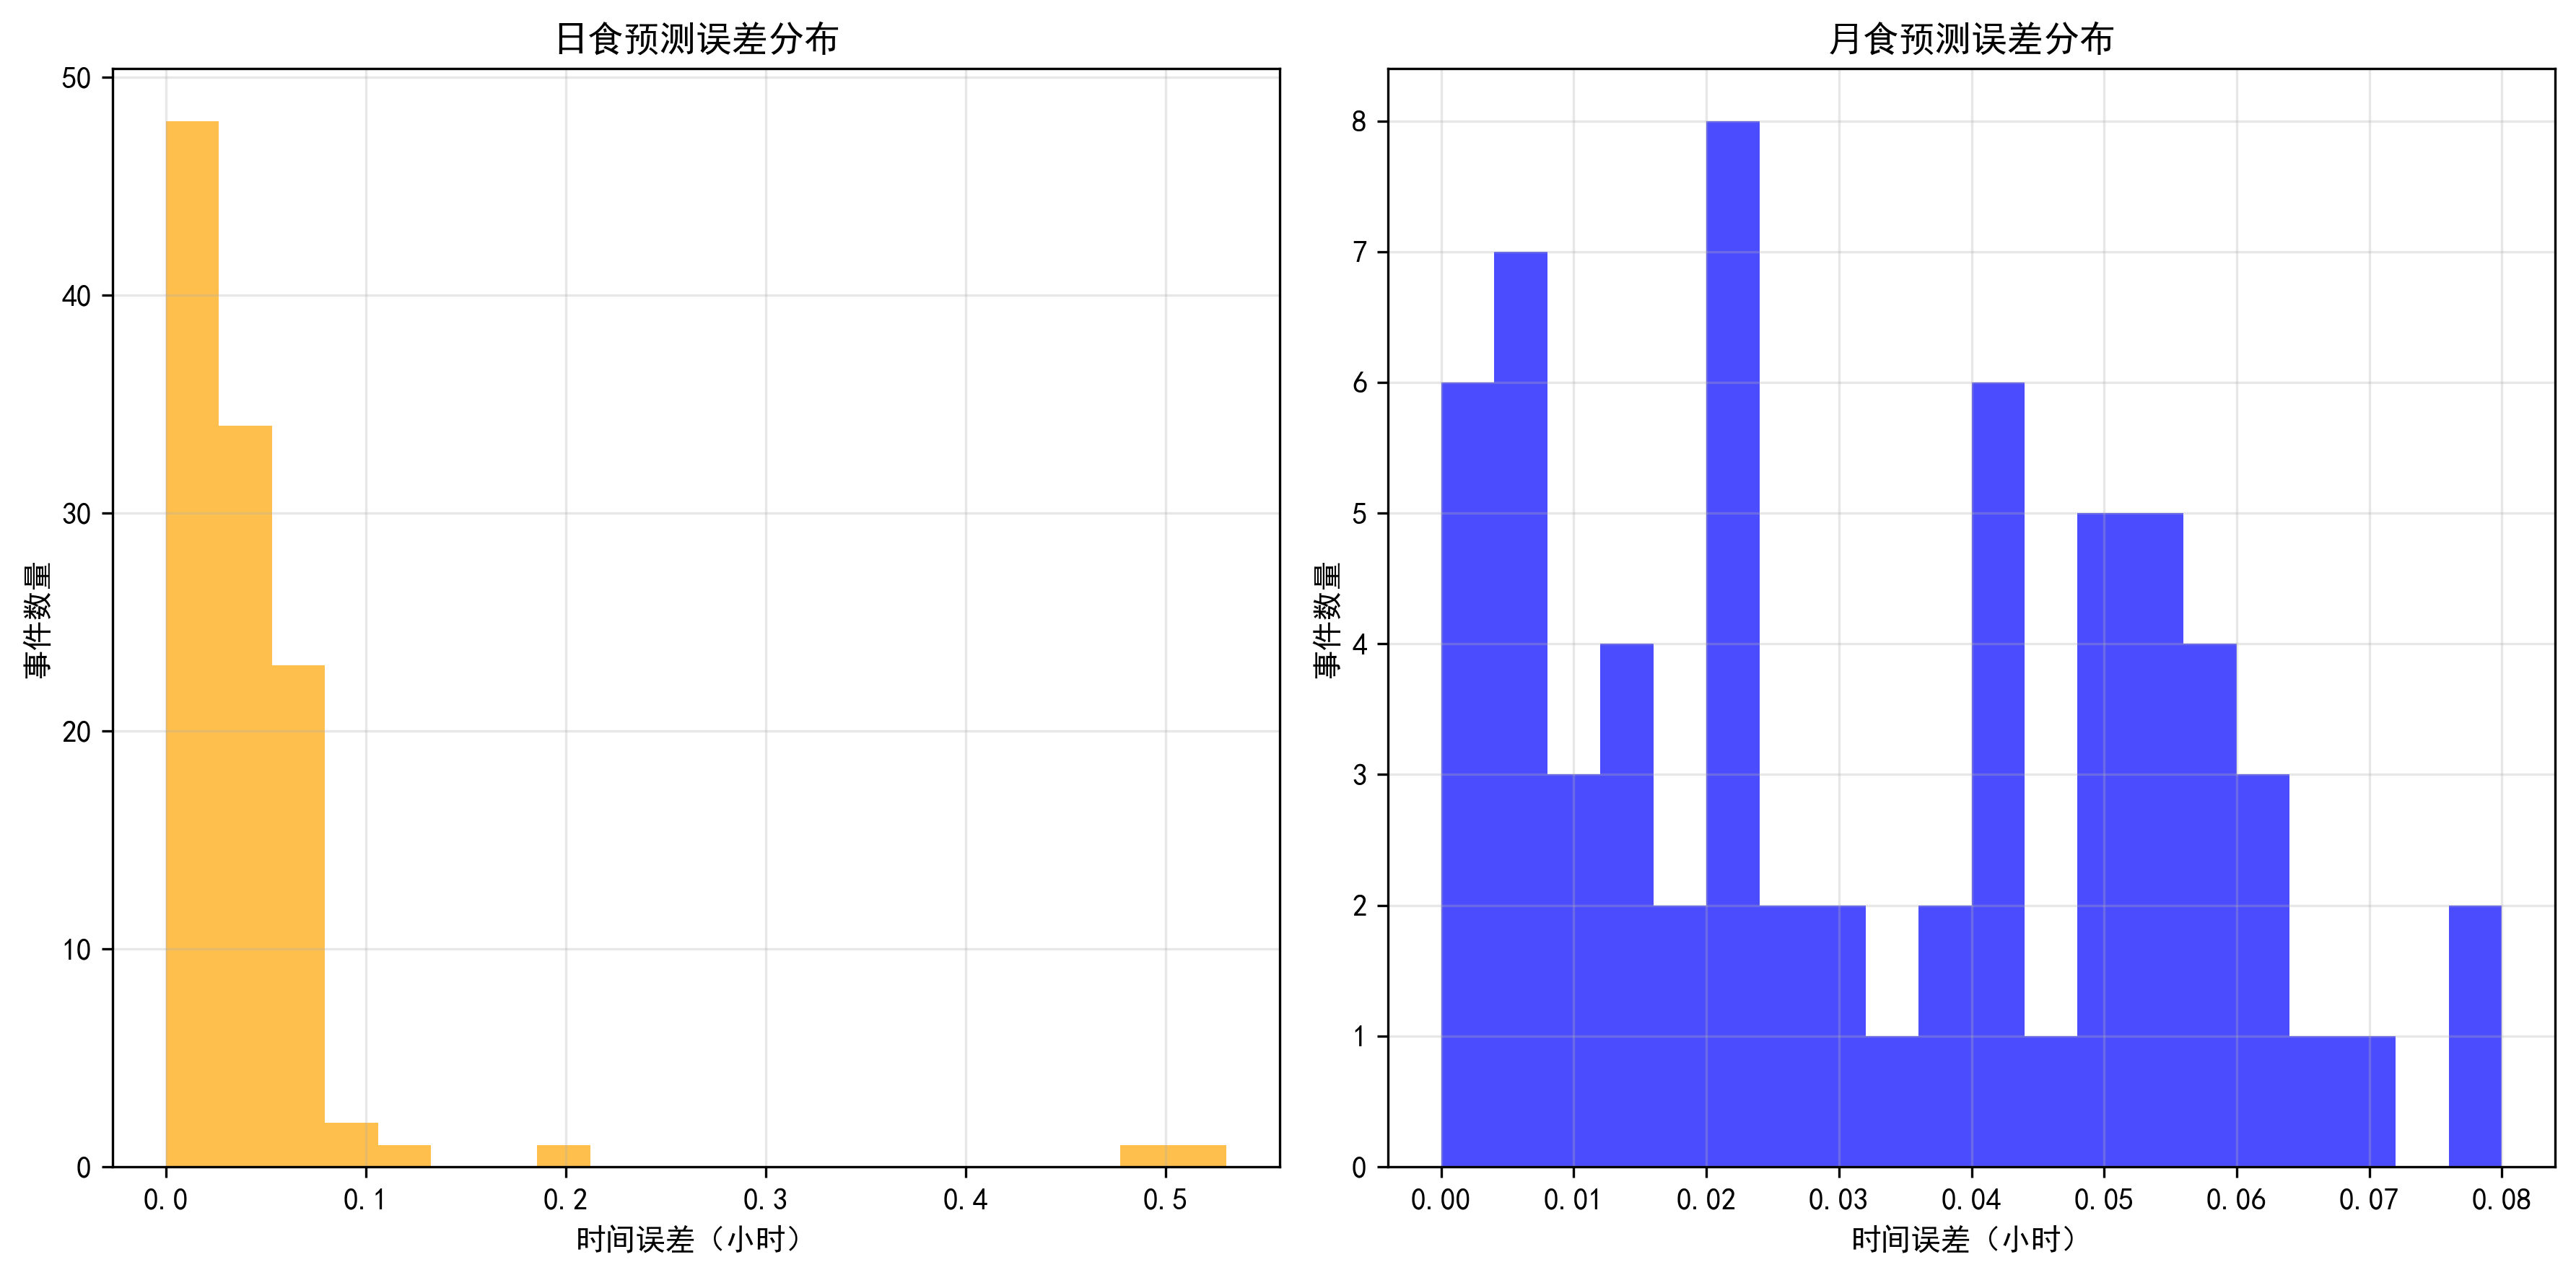
\includegraphics[width=0.5\linewidth]{images/error_distribution_earth.png}
    \caption{扰动对象:月球质量(预测准确率:96.70\%)}
    \label{fig:eclipse_error_moon}
\end{figure}

可以发现在日、地、月三者中,对最终结果影响最明显的是地球,然而比较影响后的轨道可以发现(具体数据在这里不进一步列出),对绝对位置影响最明显的是太阳的质量。
这佐证了之前应该使用最终日/月食时间误差而非天体位置作为结果优劣的评价标准。同时,由于我们使用的天体质量精度都在10位有效数字以上,无需担心来自这方面的误差。\\
最后,绘制最优的参数组合(综合考虑运行速度和精度)下的结果如图\ref{fig:eclipse_error_best}所示,可以看到预测的误差均在15min以内,绝大部分预测的误差都在10min以内。
\begin{figure}[H]
    \centering
    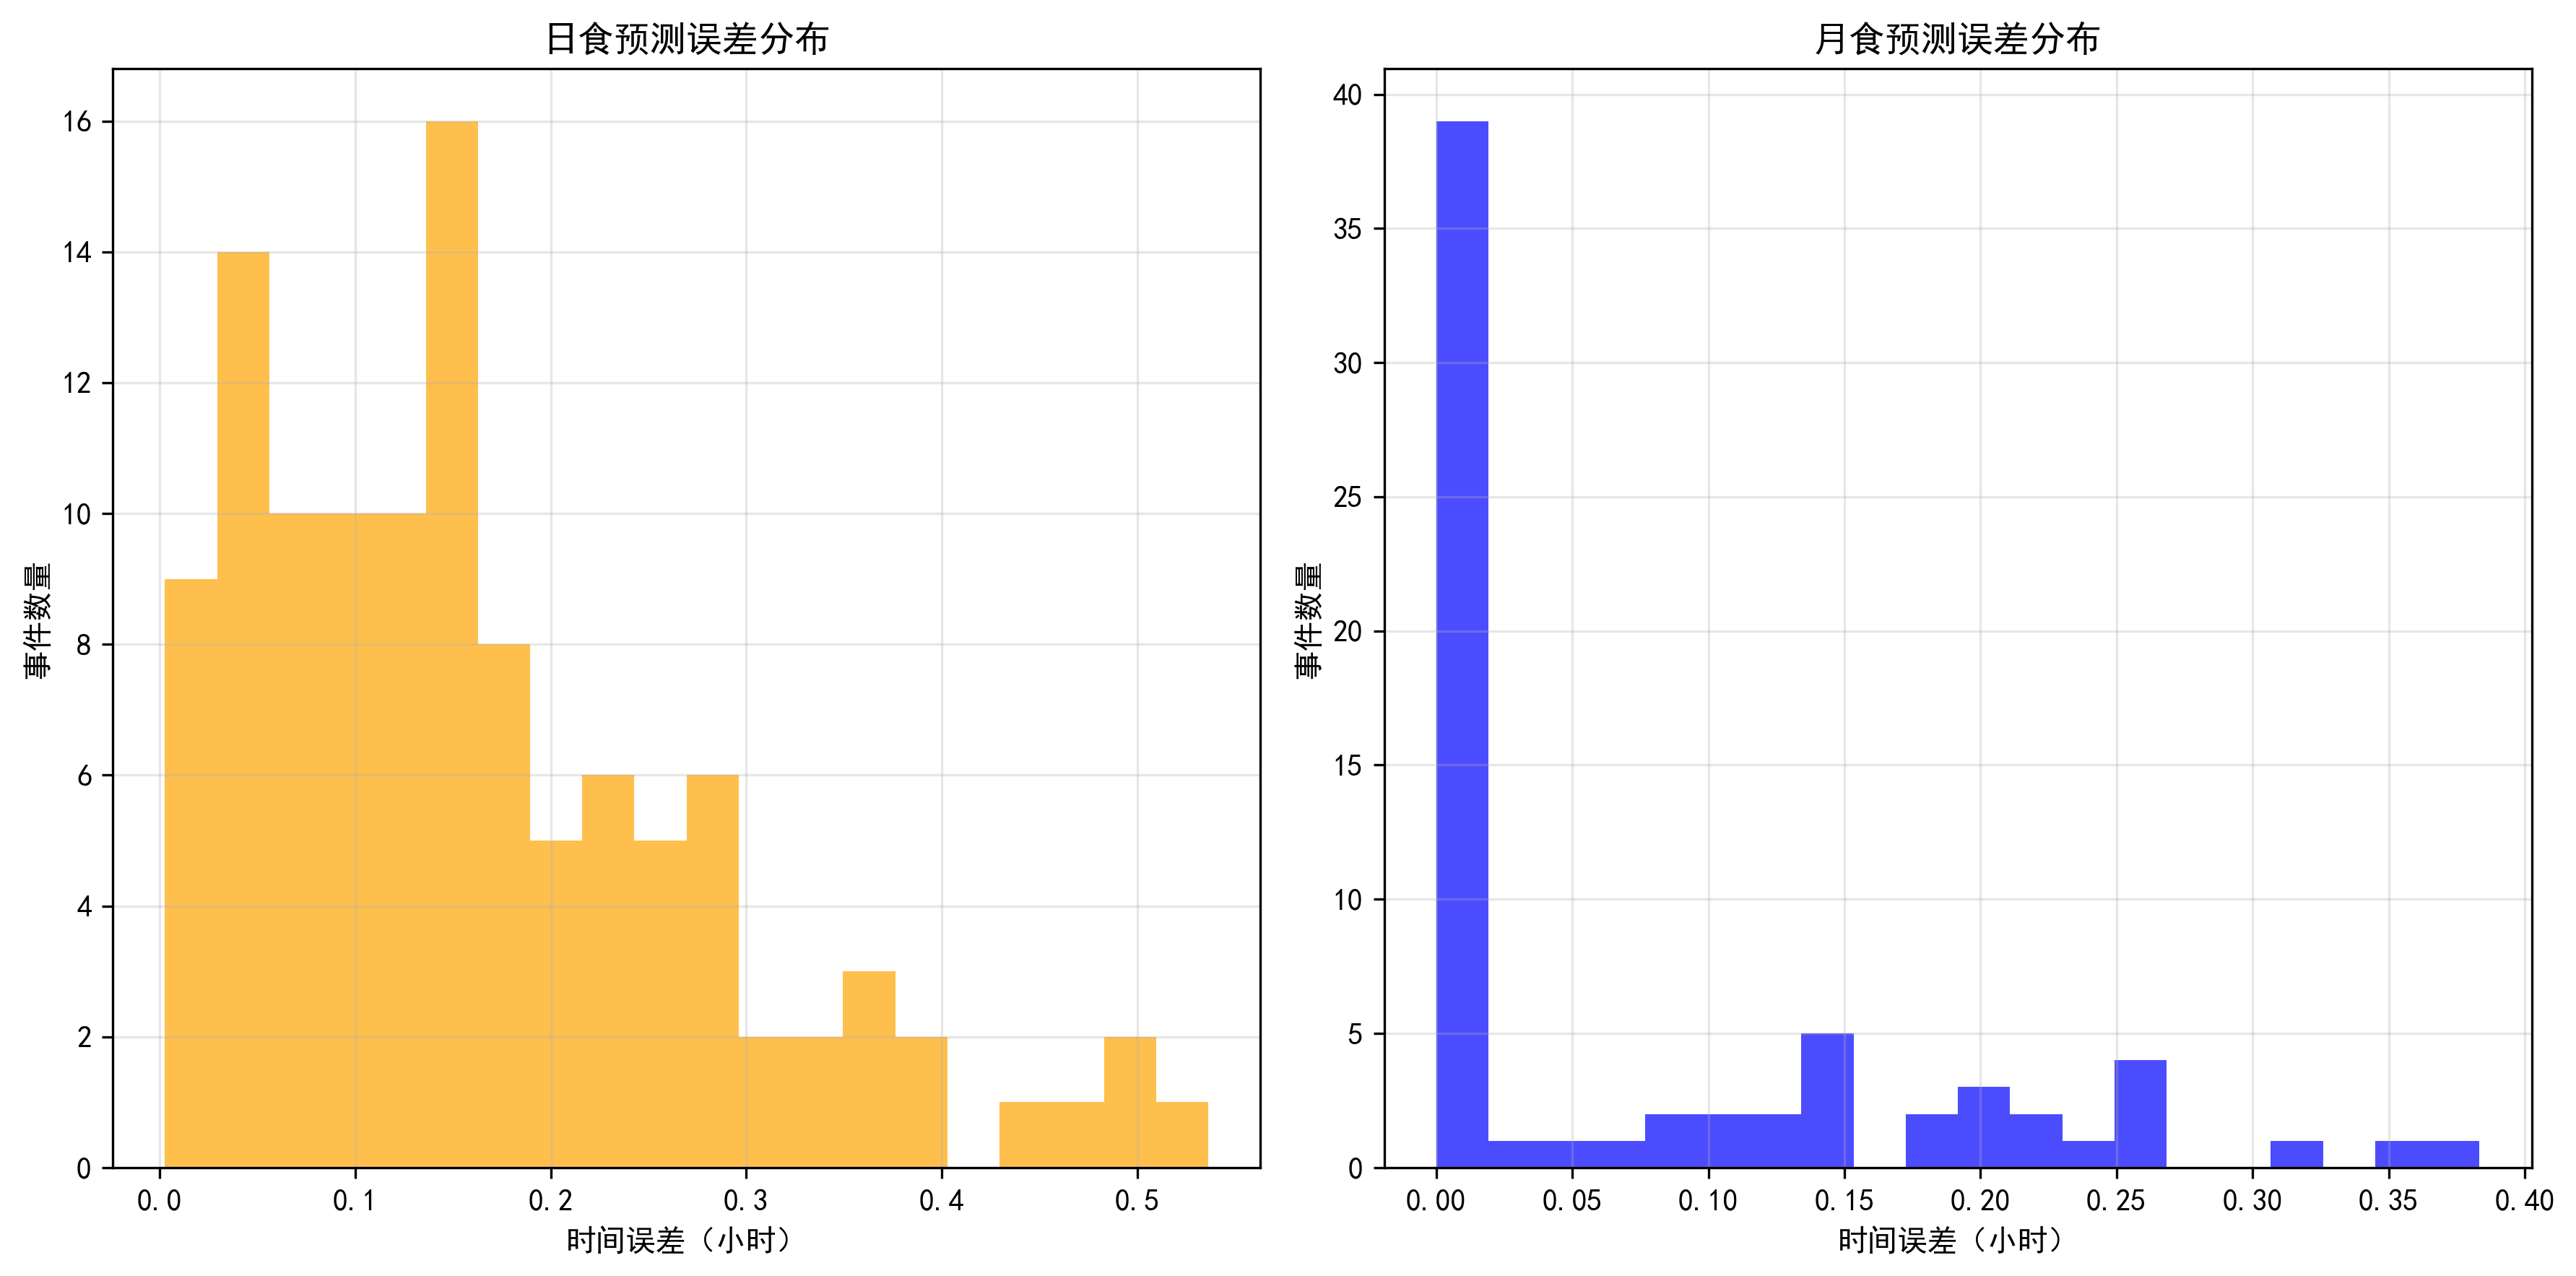
\includegraphics[width=0.5\linewidth]{images/error_distribution.png}
    \caption{最优结果(预测准确率:99.45\%)}
    \label{fig:eclipse_error_best}
\end{figure}


\section{引用}

[1] 张平文,李铁军. 数值分析 (1991,北京大学出版社)
\end{document}
